
\section{Details of mean p-value}

\label{app:rateshape_mean_pvalue}

The p-value distributions for fake datasets with different number of events
is shown in figure~\ref{fig:pvalue_mean_nevents_lowpot}
%and figure~\ref{fig:pvalue_mean_nevents_highpot} 
for
\TotalPot POT. 
%\FakePotLow POT and \FakePotHigh POT.

\begin{figure}
\center
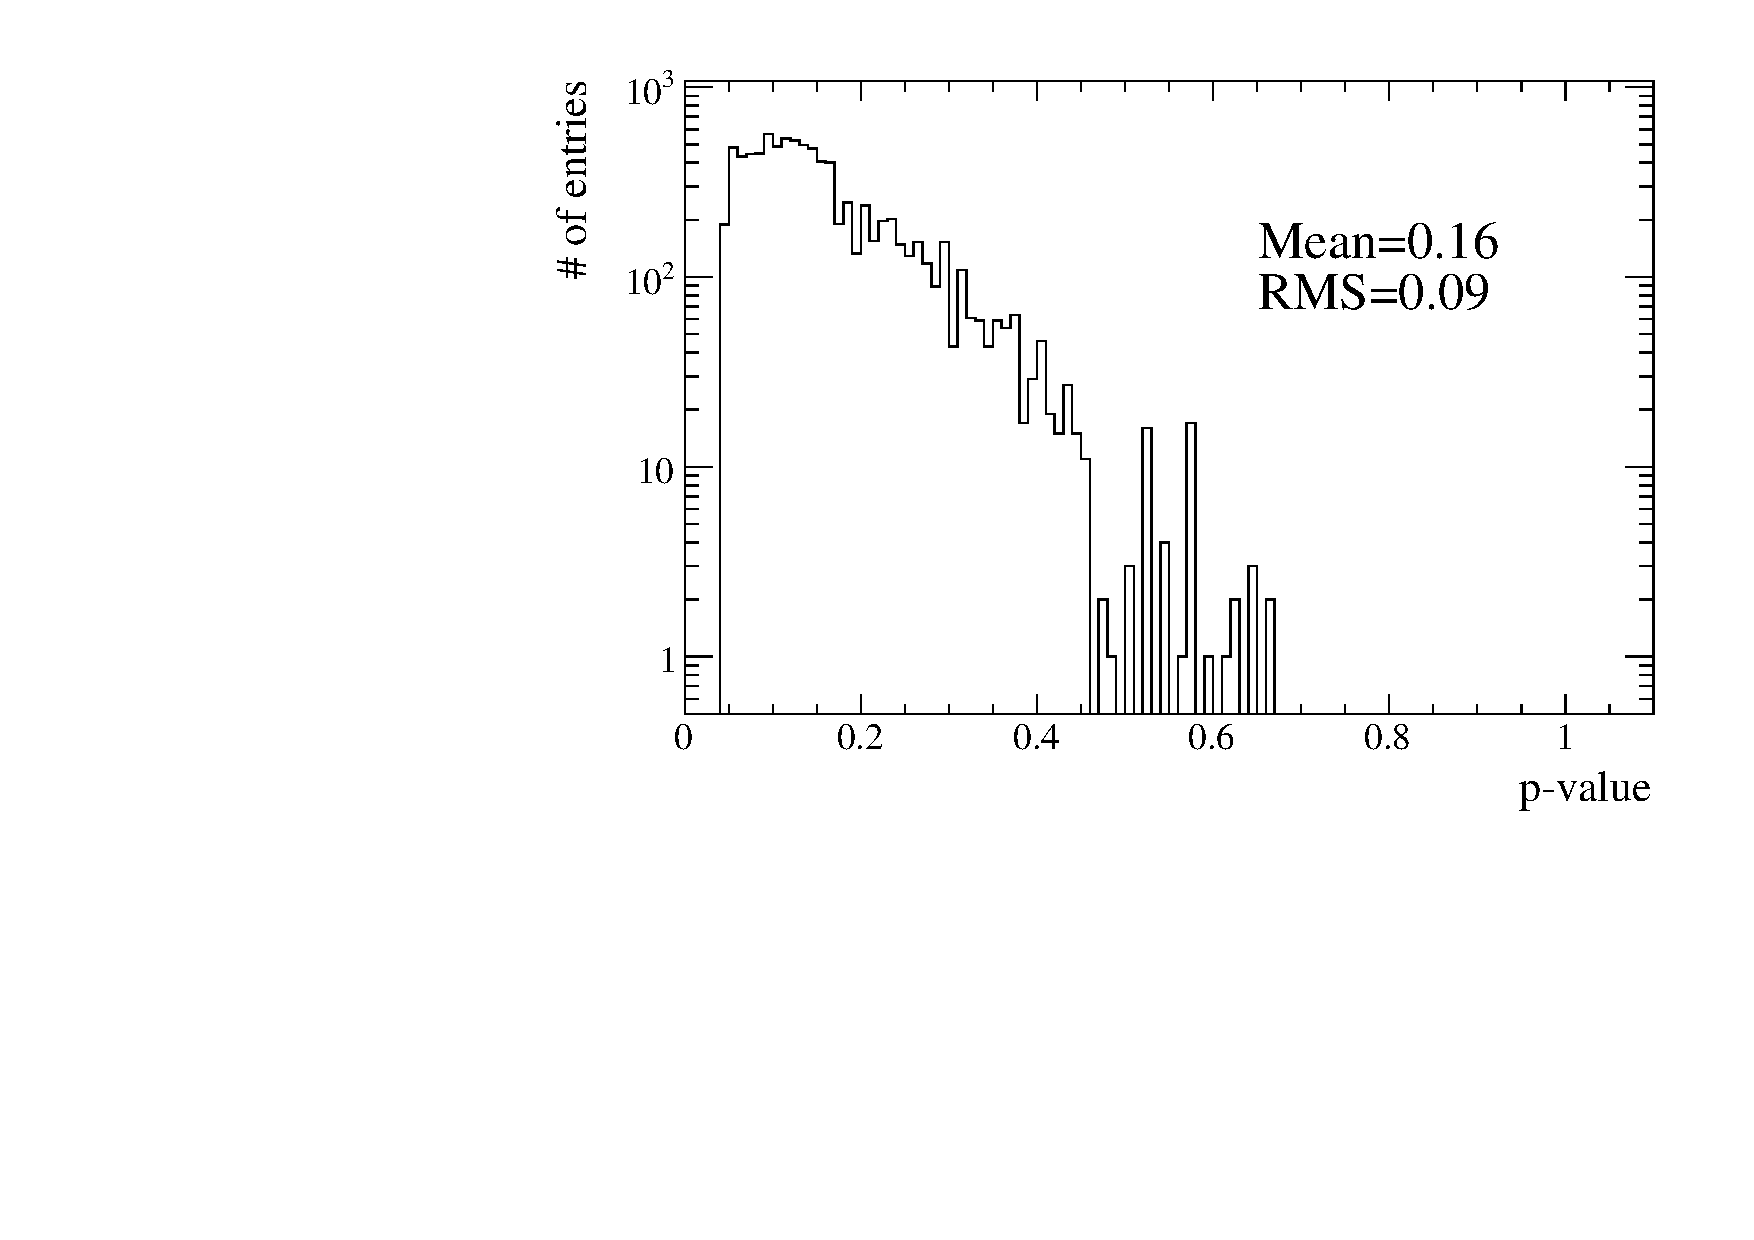
\includegraphics[width=0.48\linewidth]{./nuebar_plots/pvalue_mean/pvalue_rateshape_ave_3evt_4p0108E20POT_50ktoys.pdf}
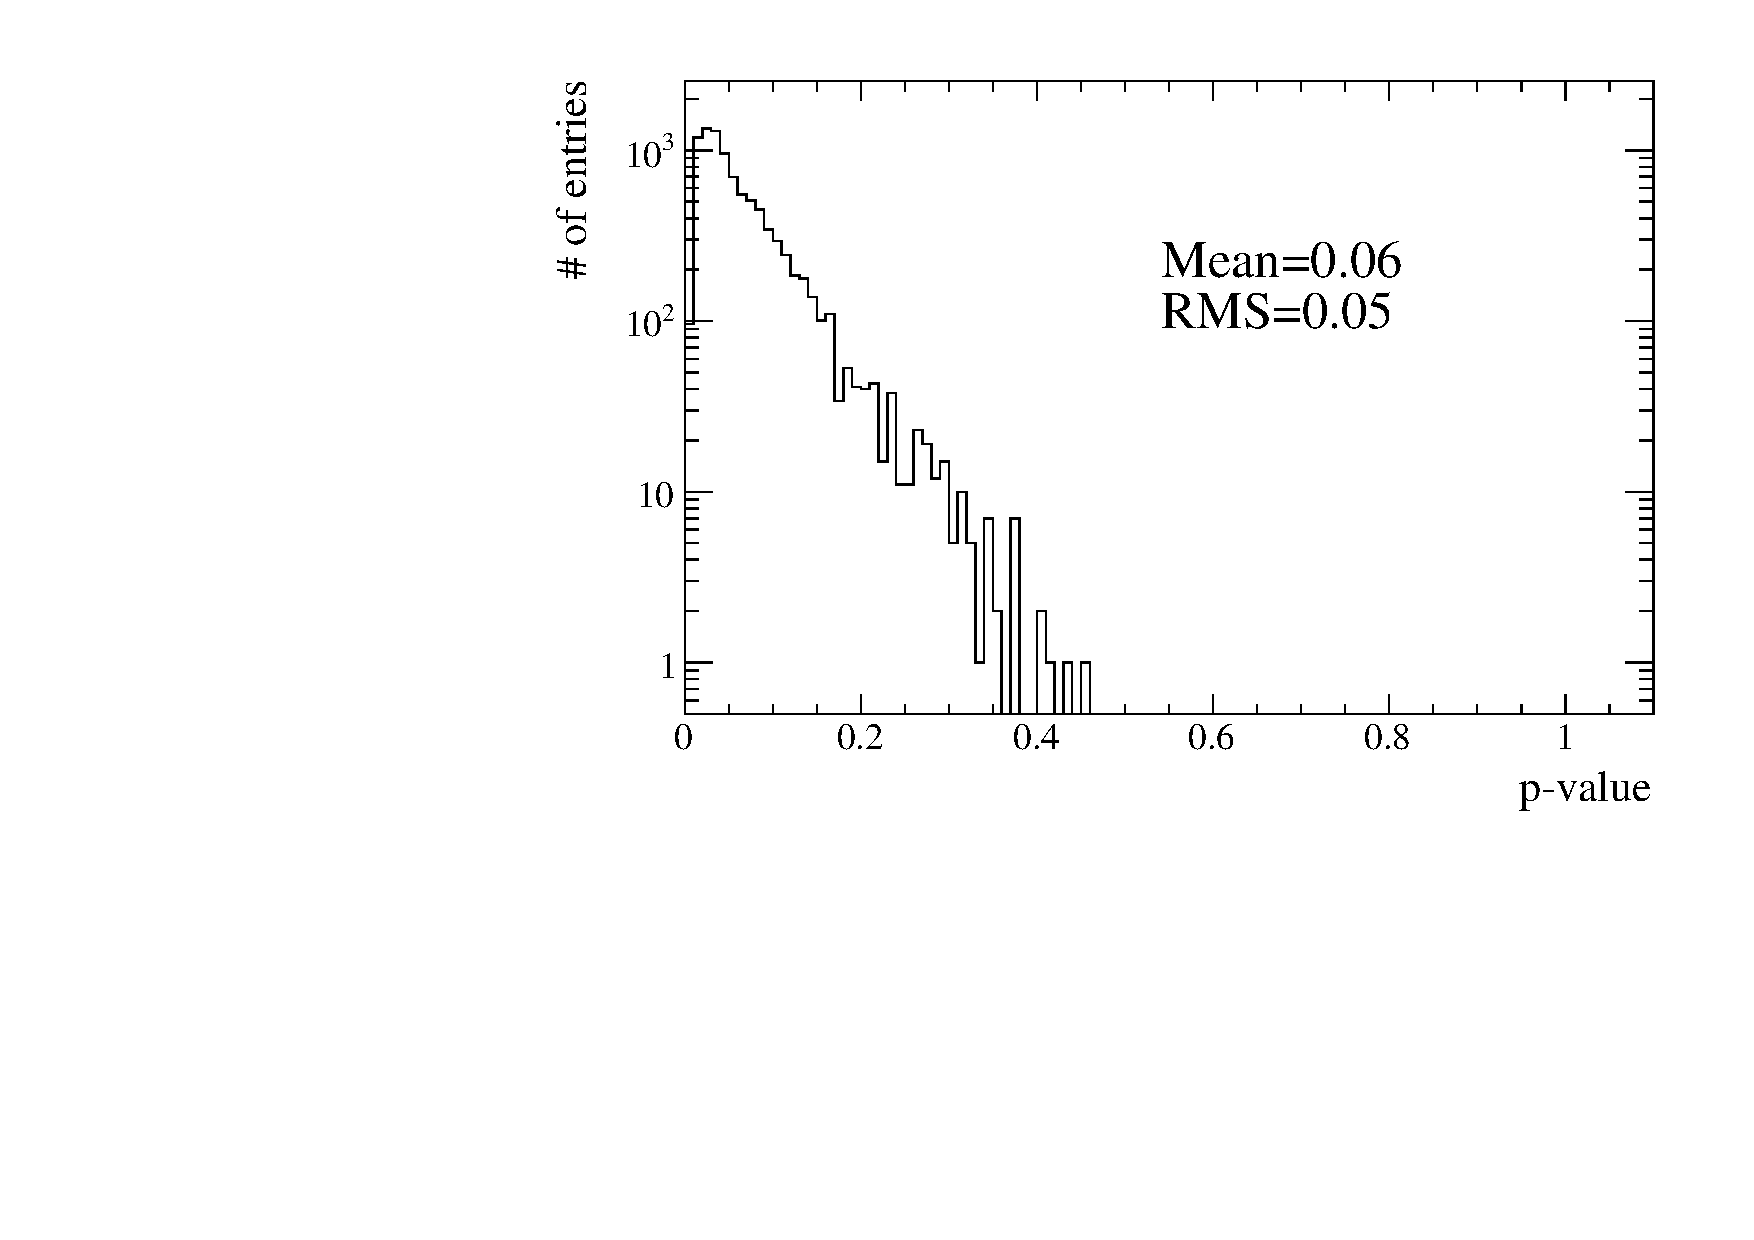
\includegraphics[width=0.48\linewidth]{./nuebar_plots/pvalue_mean/pvalue_rateshape_ave_4evt_4p0108E20POT_50ktoys.pdf}
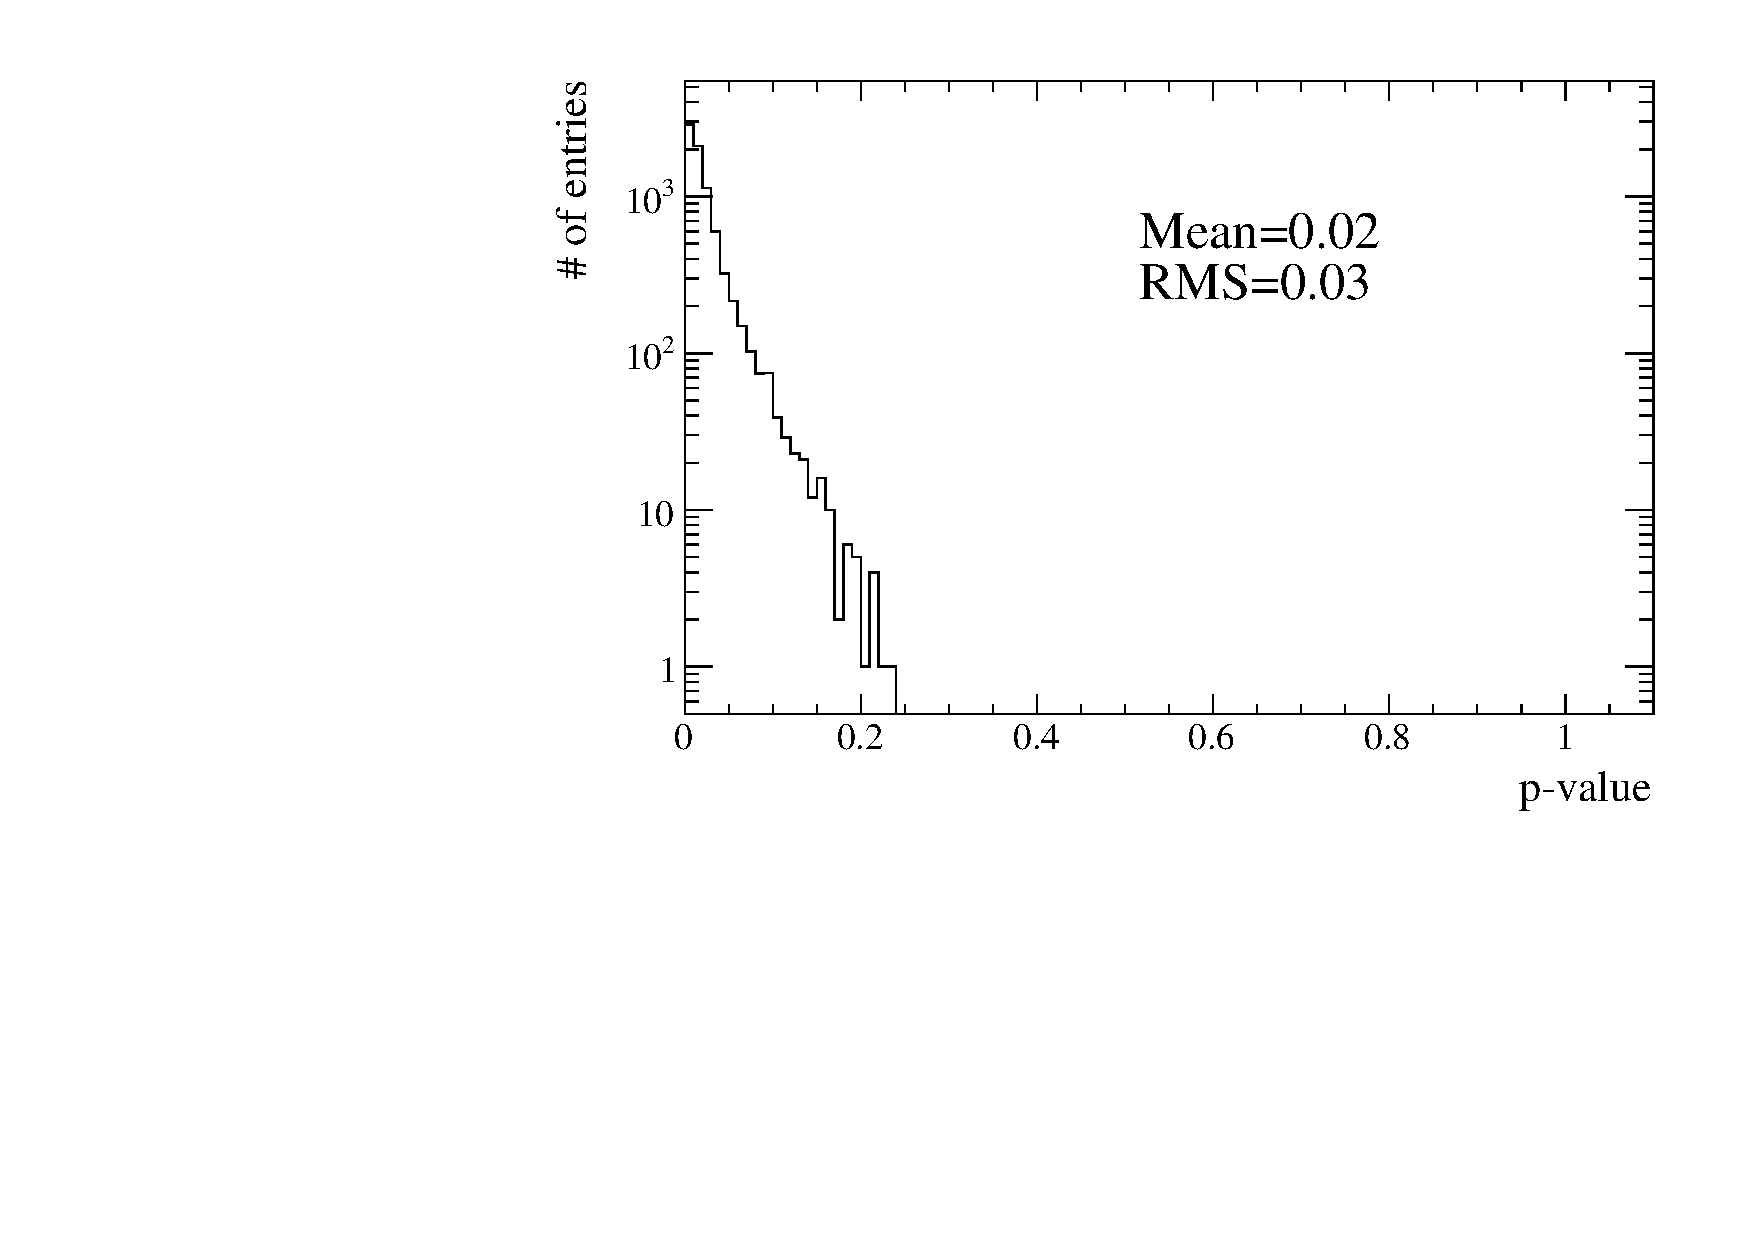
\includegraphics[width=0.48\linewidth]{./nuebar_plots/pvalue_mean/pvalue_rateshape_ave_5evt_4p0108E20POT_50ktoys.pdf}
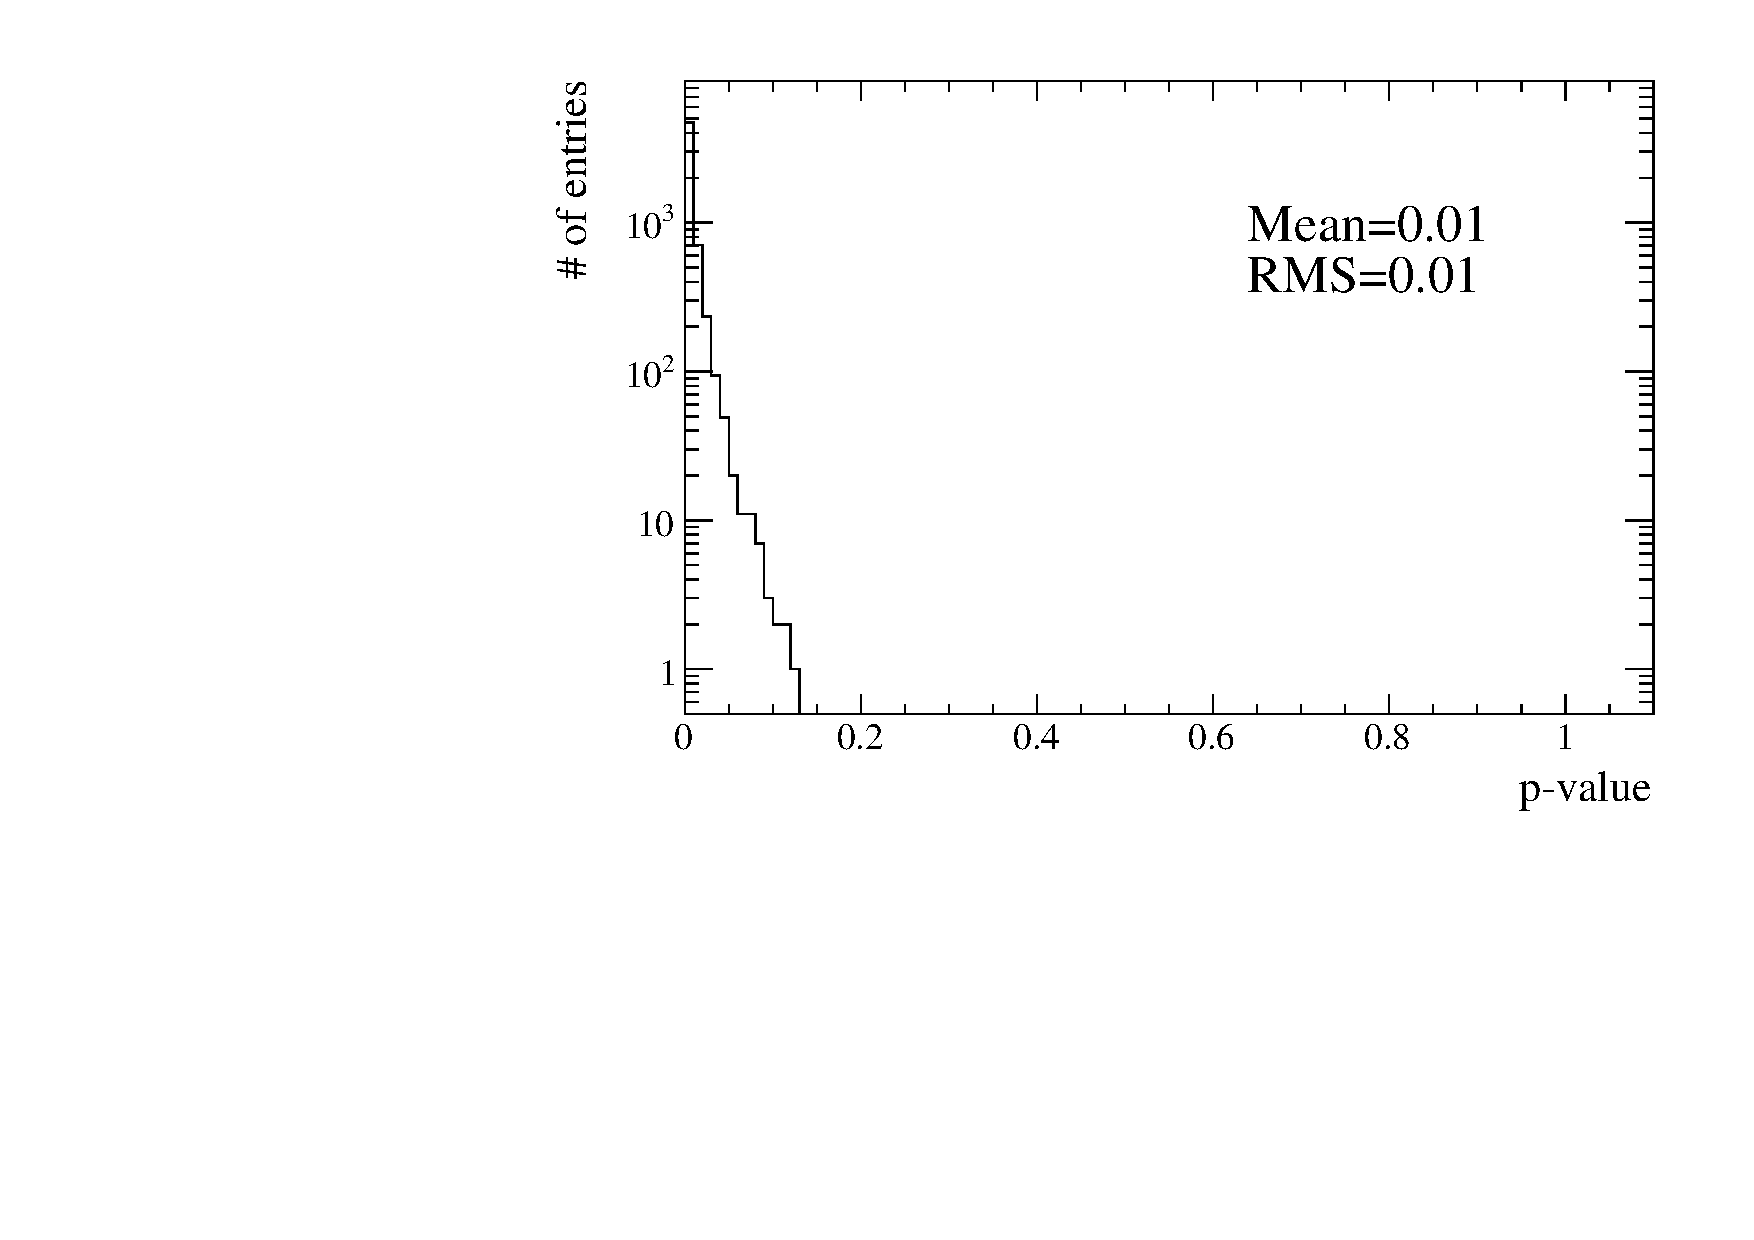
\includegraphics[width=0.48\linewidth]{./nuebar_plots/pvalue_mean/pvalue_rateshape_ave_6evt_4p0108E20POT_50ktoys.pdf}
\caption {
Distributions of the p-value corresponding to fake datasets with different number of events,
respectively from left to right and top to bottom 3, 4, 5 and 6 events.
The procedure used to obtain the p-value distributions is shown in~\ref{subsec:pvalue_mean}.
The study is performed with 
\TotalPot POT.
%\FakePotLow POT.
\NumToysLarge toys are used.
}
\label{fig:pvalue_mean_nevents_lowpot}
\end{figure}

%\begin{figure}
%\center
%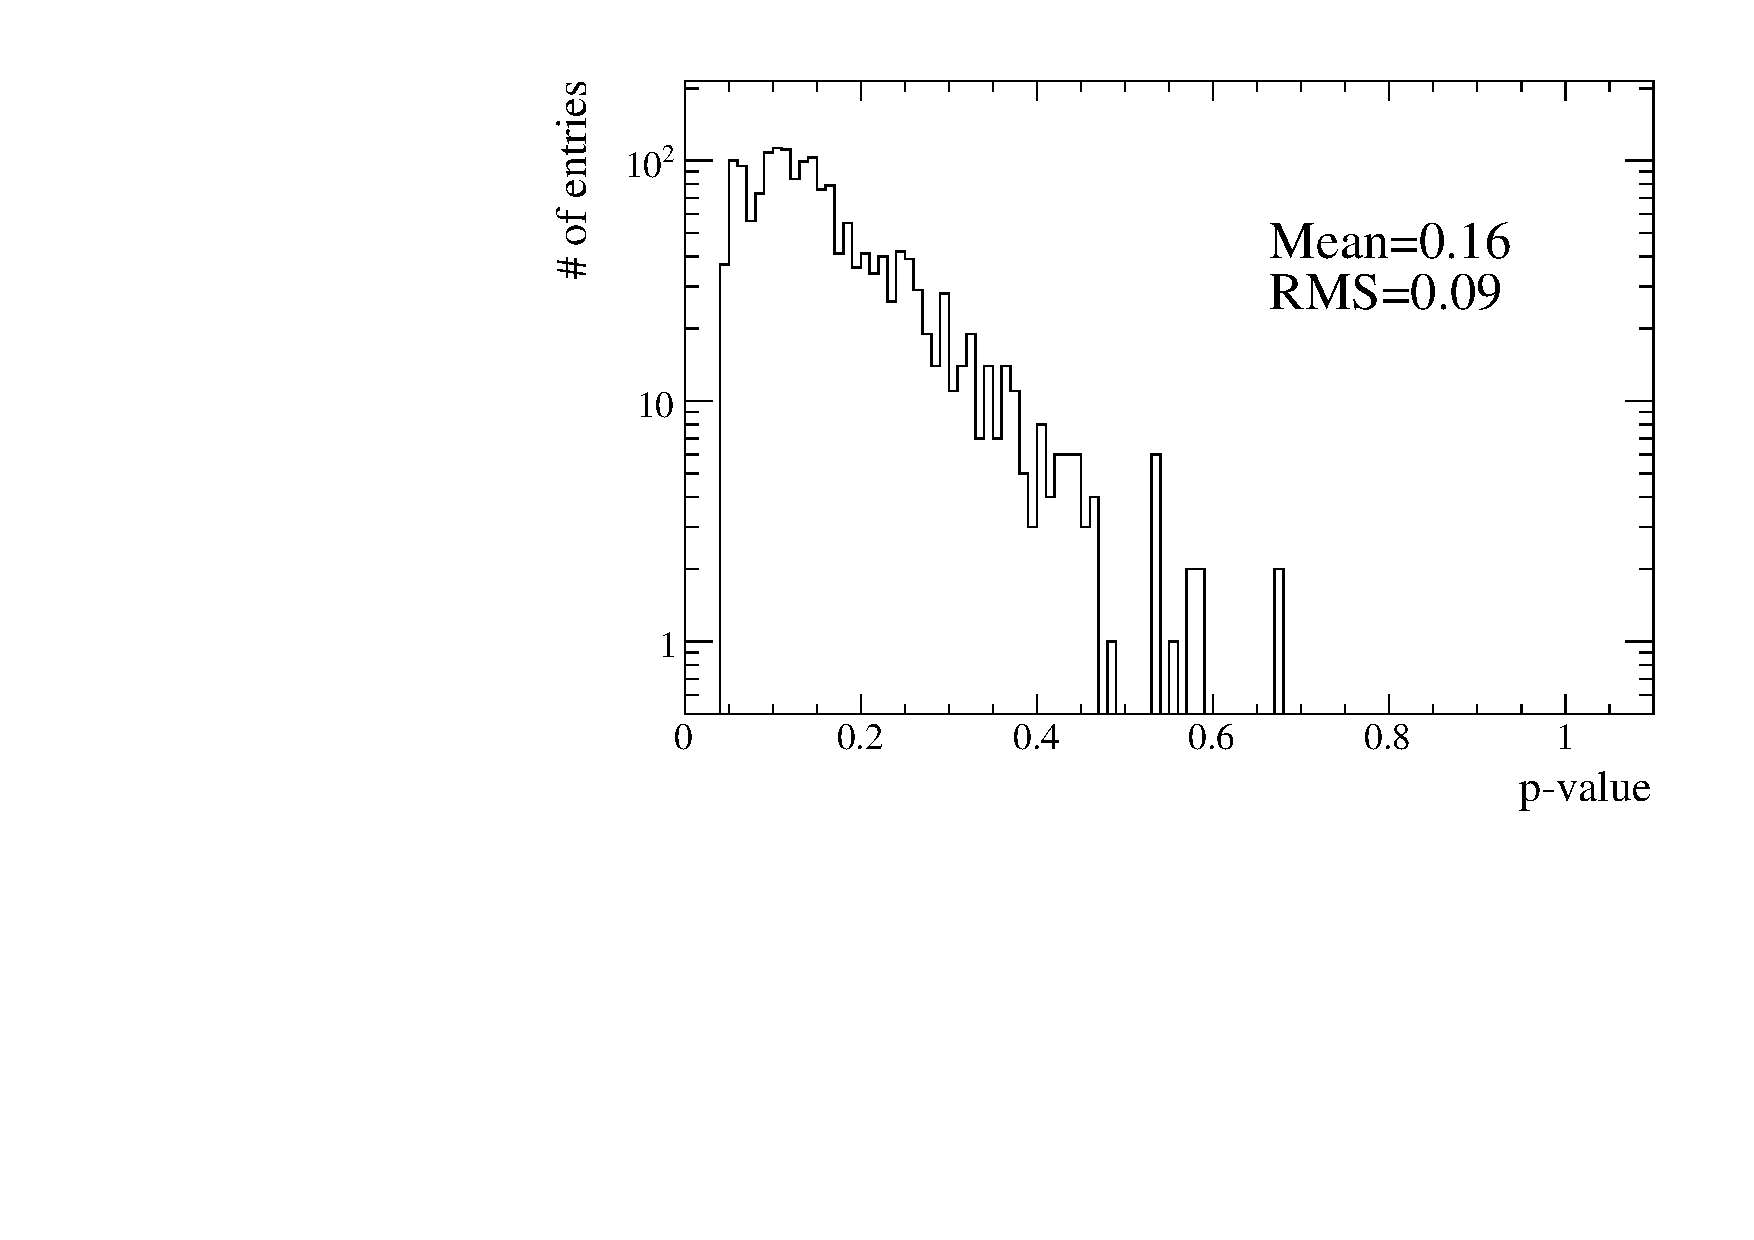
\includegraphics[width=0.48\linewidth]{./nuebar_plots/pvalue_mean/pvalue_rateshape_ave_3evt_4p5E20POT.pdf}
%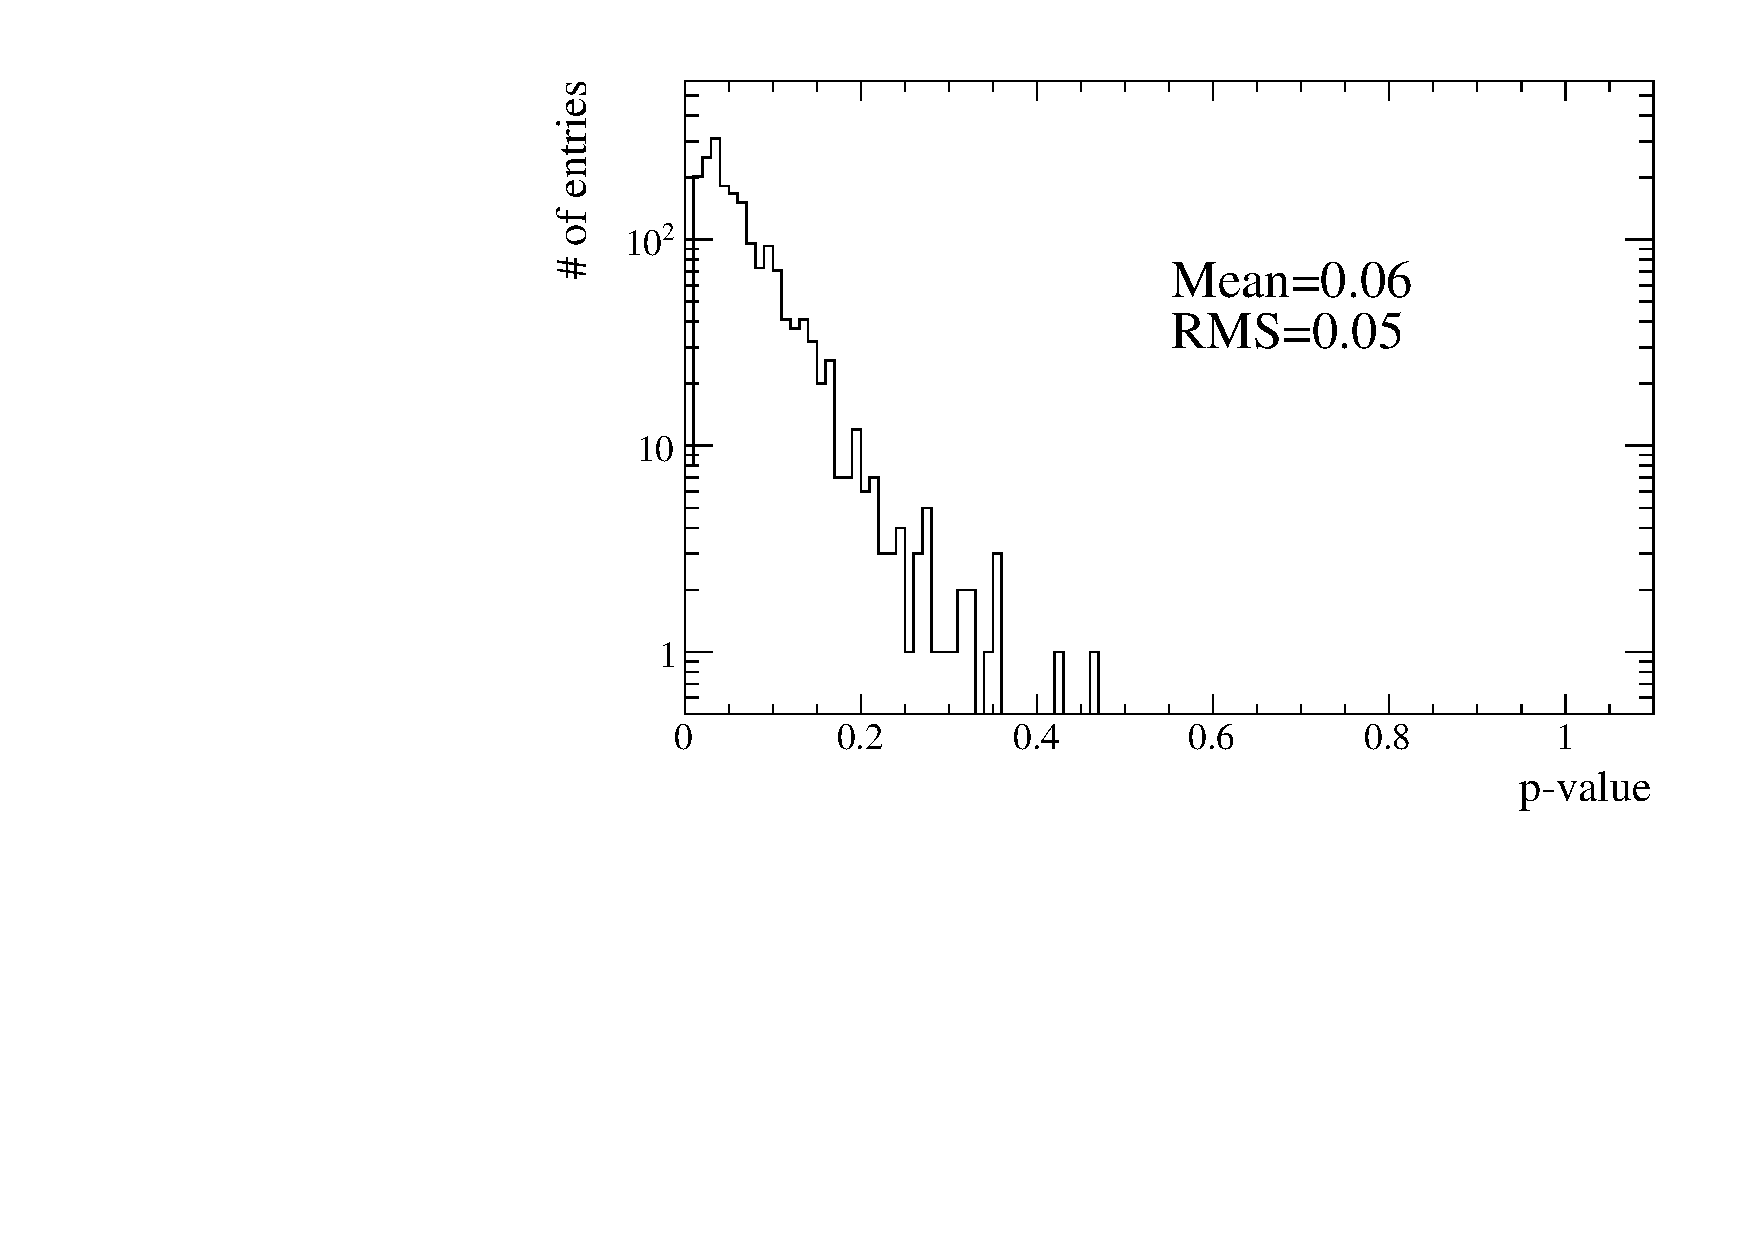
\includegraphics[width=0.48\linewidth]{./nuebar_plots/pvalue_mean/pvalue_rateshape_ave_4evt_4p5E20POT.pdf}
%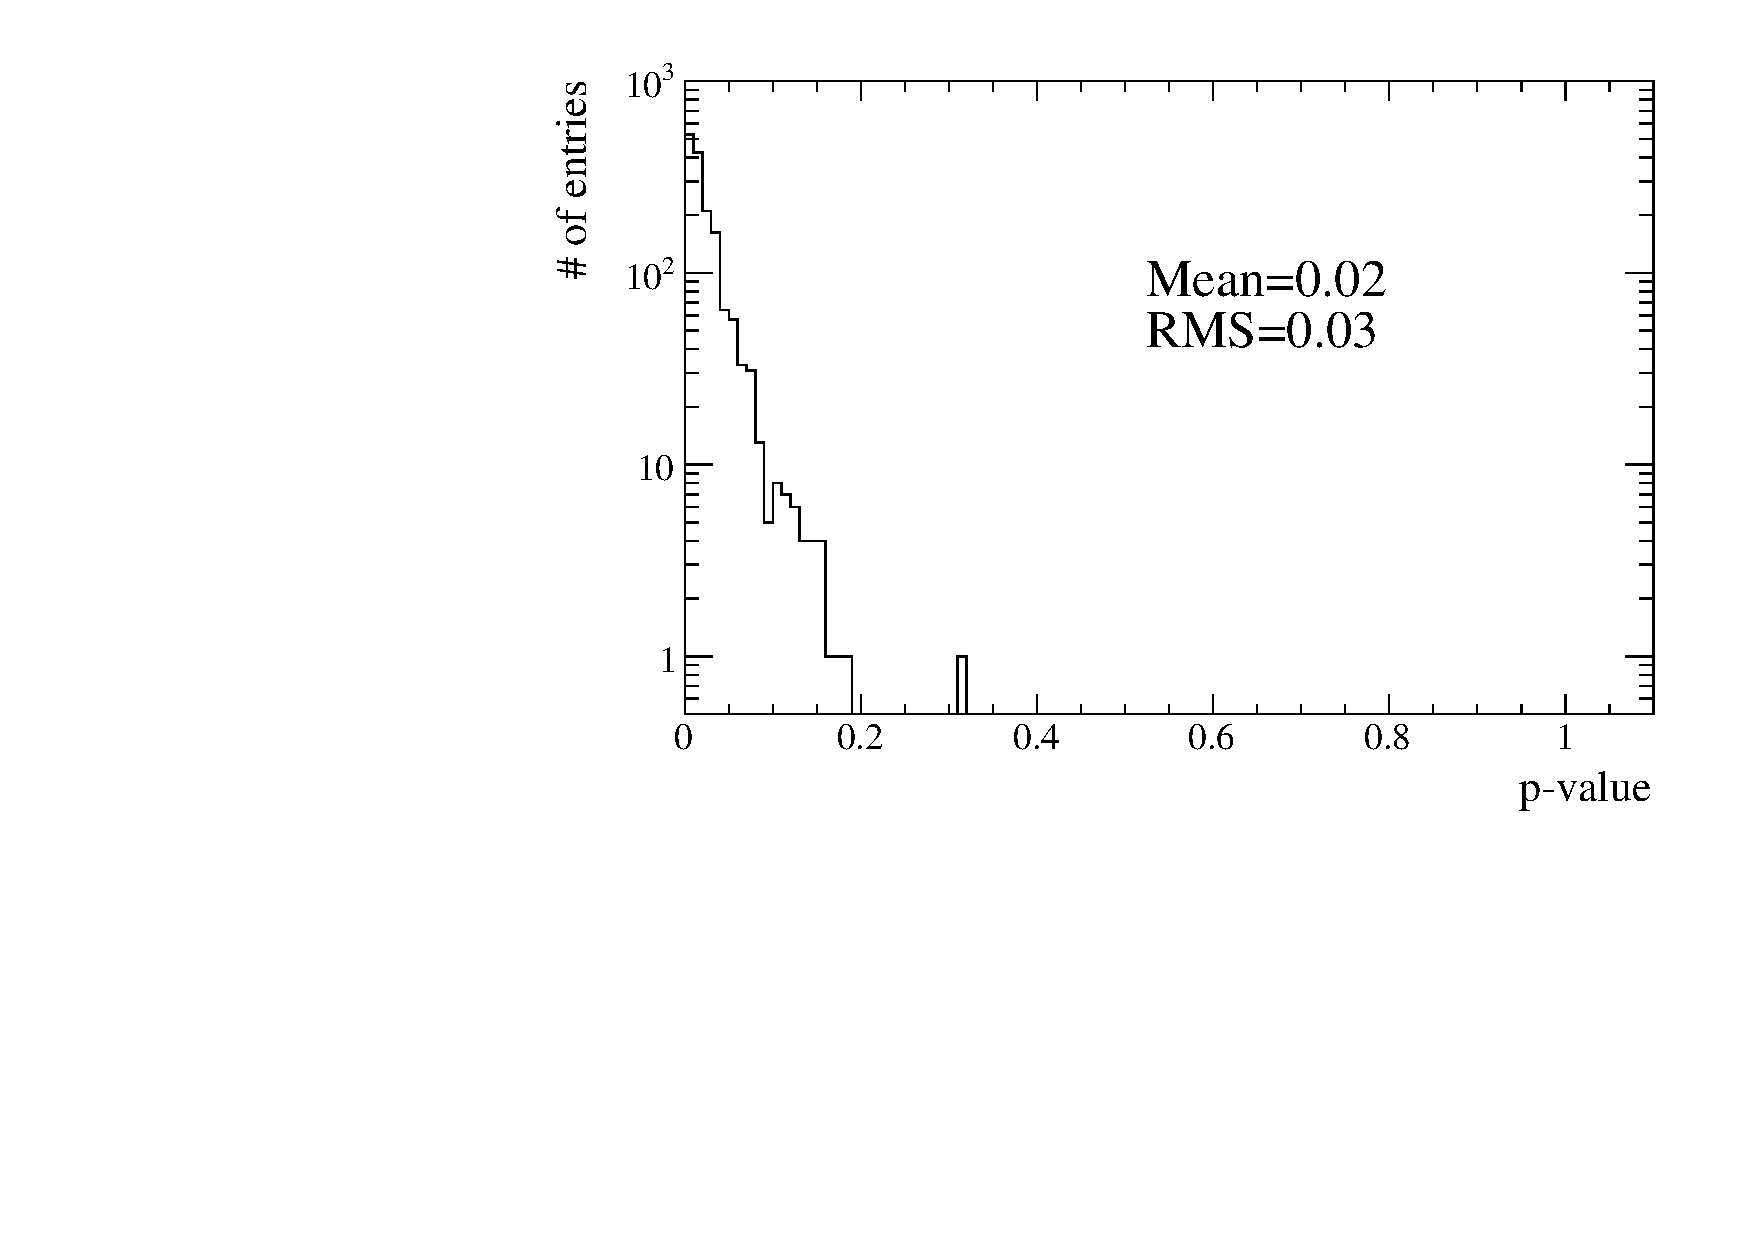
\includegraphics[width=0.48\linewidth]{./nuebar_plots/pvalue_mean/pvalue_rateshape_ave_5evt_4p5E20POT.pdf}
%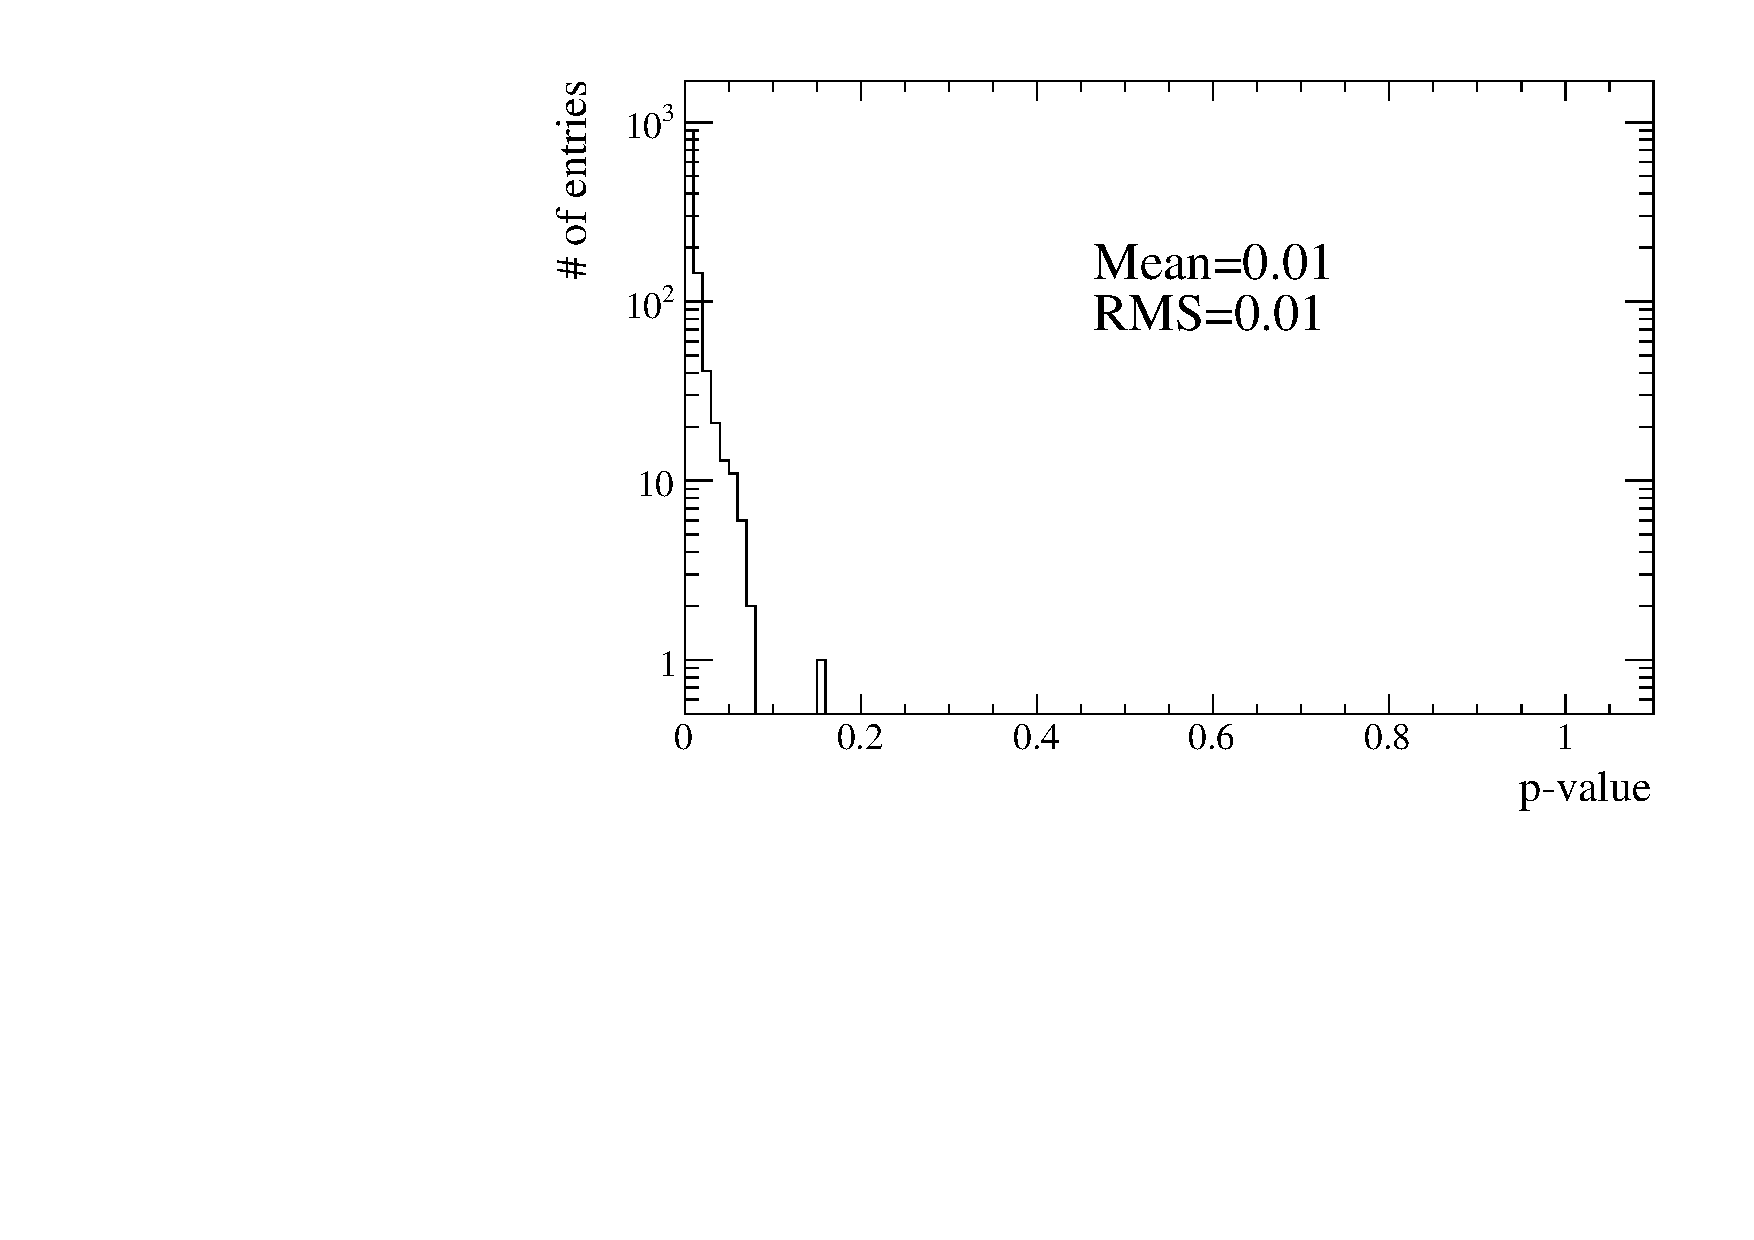
\includegraphics[width=0.48\linewidth]{./nuebar_plots/pvalue_mean/pvalue_rateshape_ave_6evt_4p5E20POT.pdf}
%\caption {
%Distributions of the p-value corresponding to fake datasets with different number of events,
%respectively from left to right and top to bottom 3, 4, 5 and 6 events.
%The procedure used to obtain the p-value distributions is shown in~\ref{subsec:pvalue_mean}.
%The study is performed with \FakePotHigh POT.
%}
%\label{fig:pvalue_mean_nevents_highpot}
%\end{figure}


The mean rate-only and rate+shape p-values, obtained considering only p-values smaller than 0.05 (0.10), 
are shown table~\ref{fig:pvalue_mean_0p05_lowpot}.
% and in table~\ref{fig:pvalue_mean_0p05_highpot}.

\begin{figure}
\center
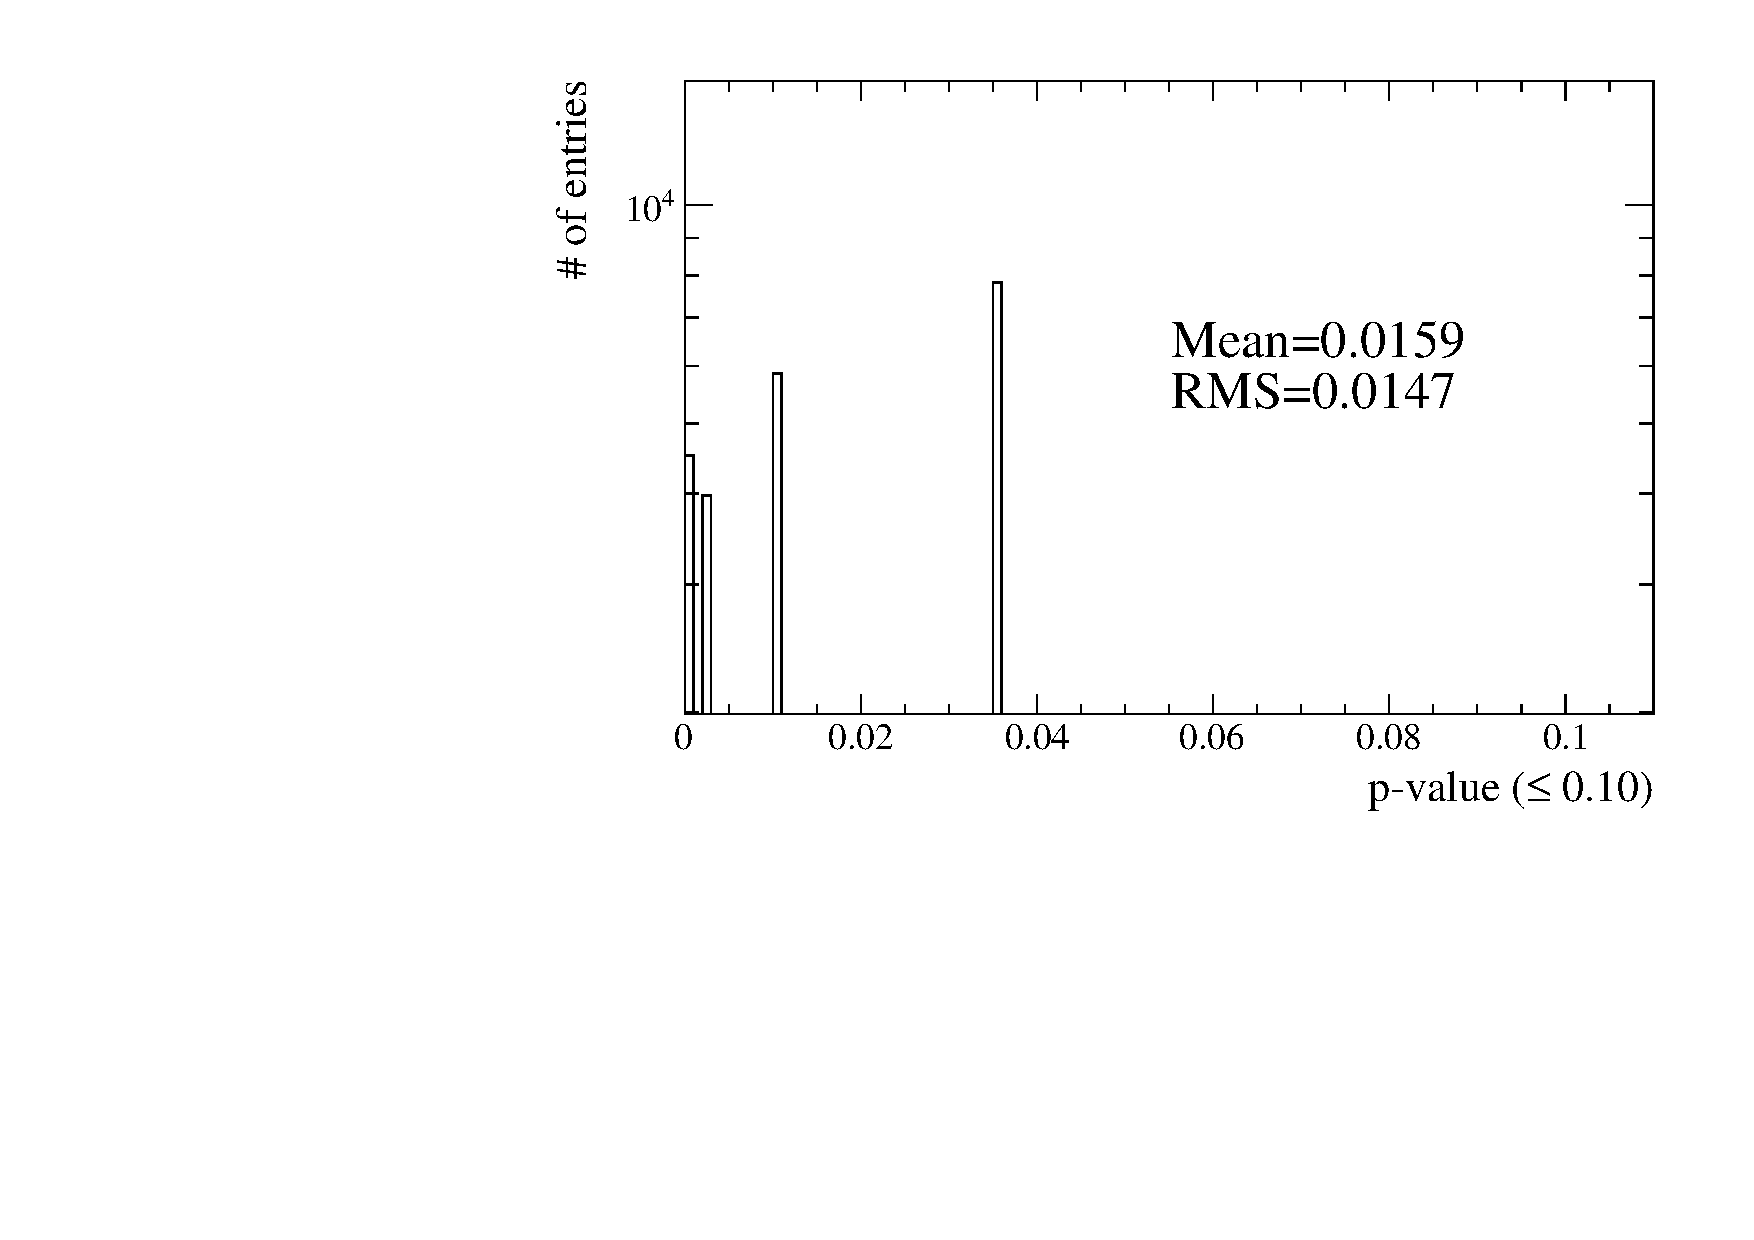
\includegraphics[width=0.48\linewidth]{./nuebar_plots/pvalue_mean/pvalue_fraction_4p0108E20POT/pvalue_rateonly_0p10_4p0108E20POT_50ktoys.pdf}
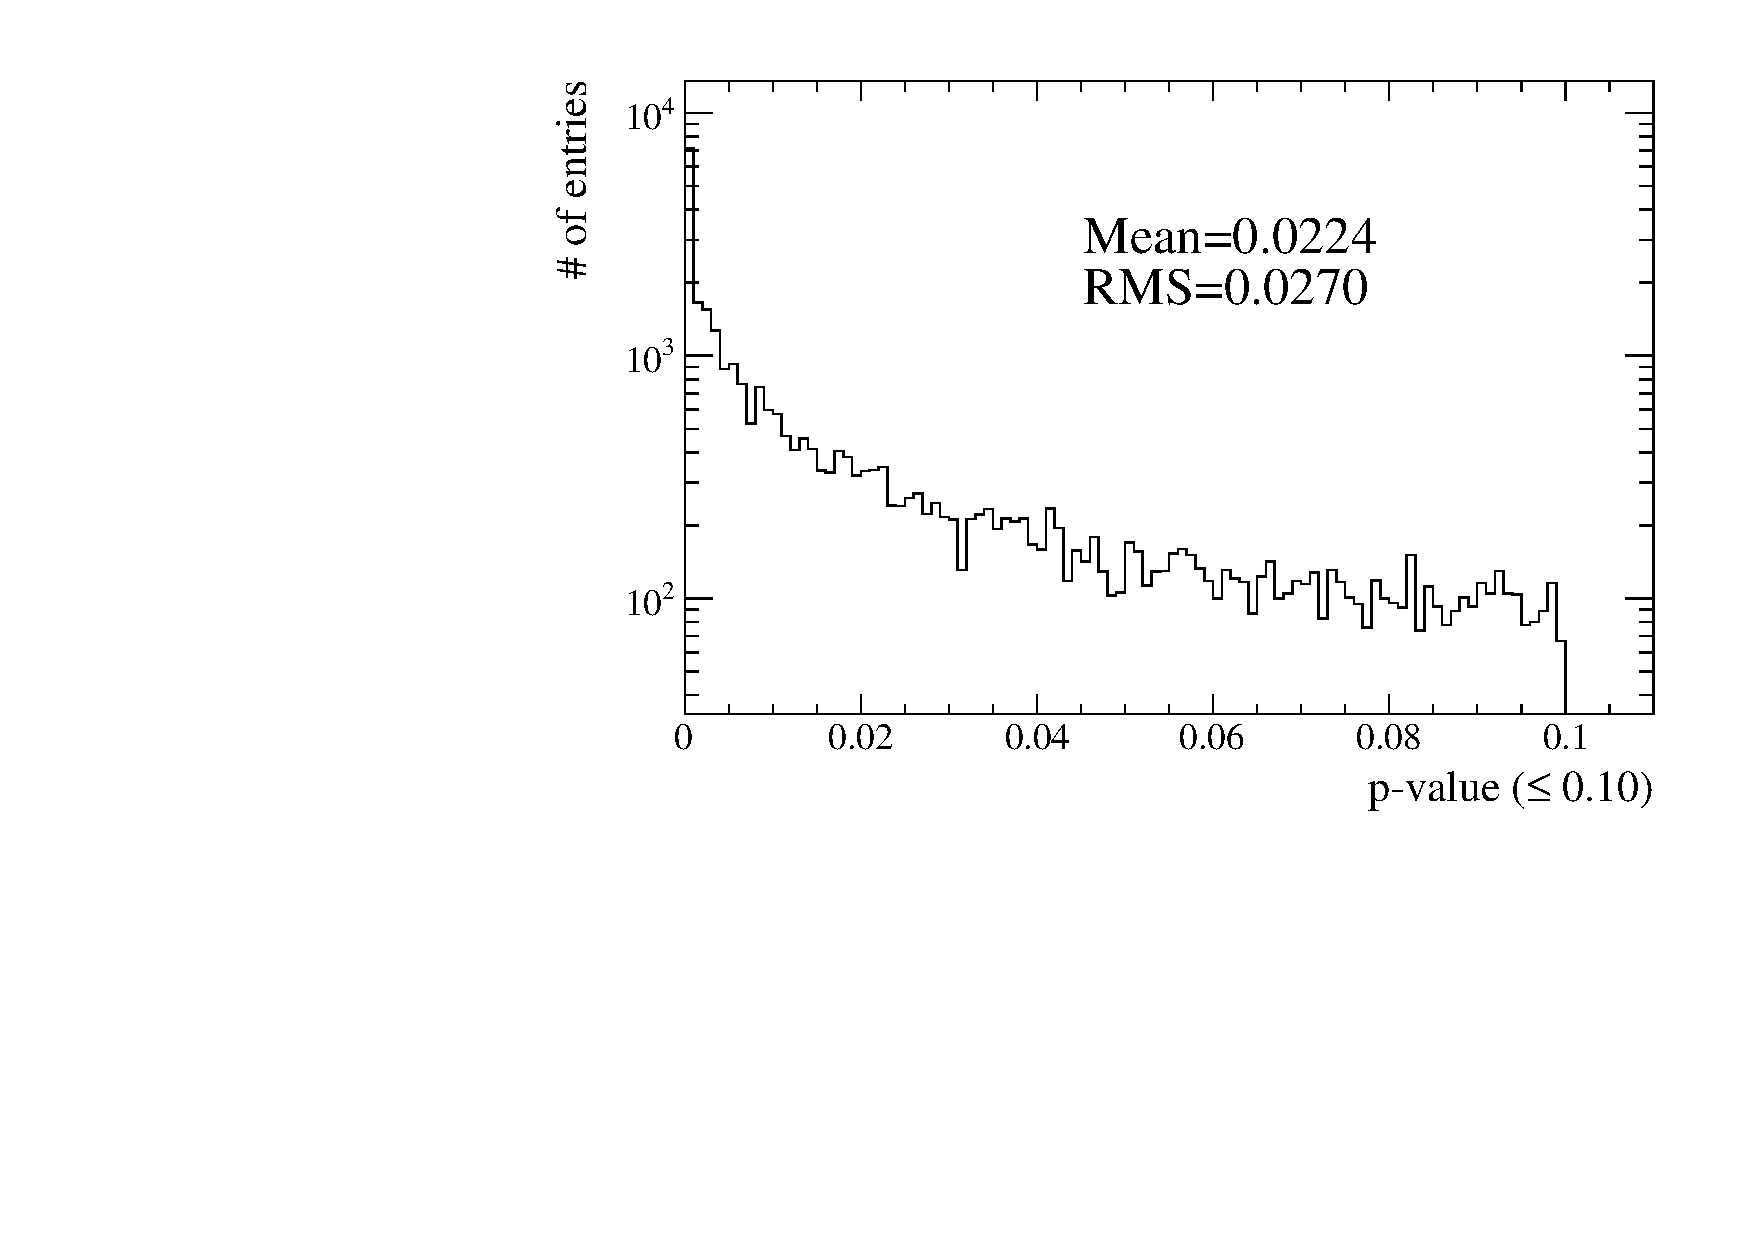
\includegraphics[width=0.48\linewidth]{./nuebar_plots/pvalue_mean/pvalue_fraction_4p0108E20POT/pvalue_rateshape_0p10_4p0108E20POT_50ktoys.pdf}
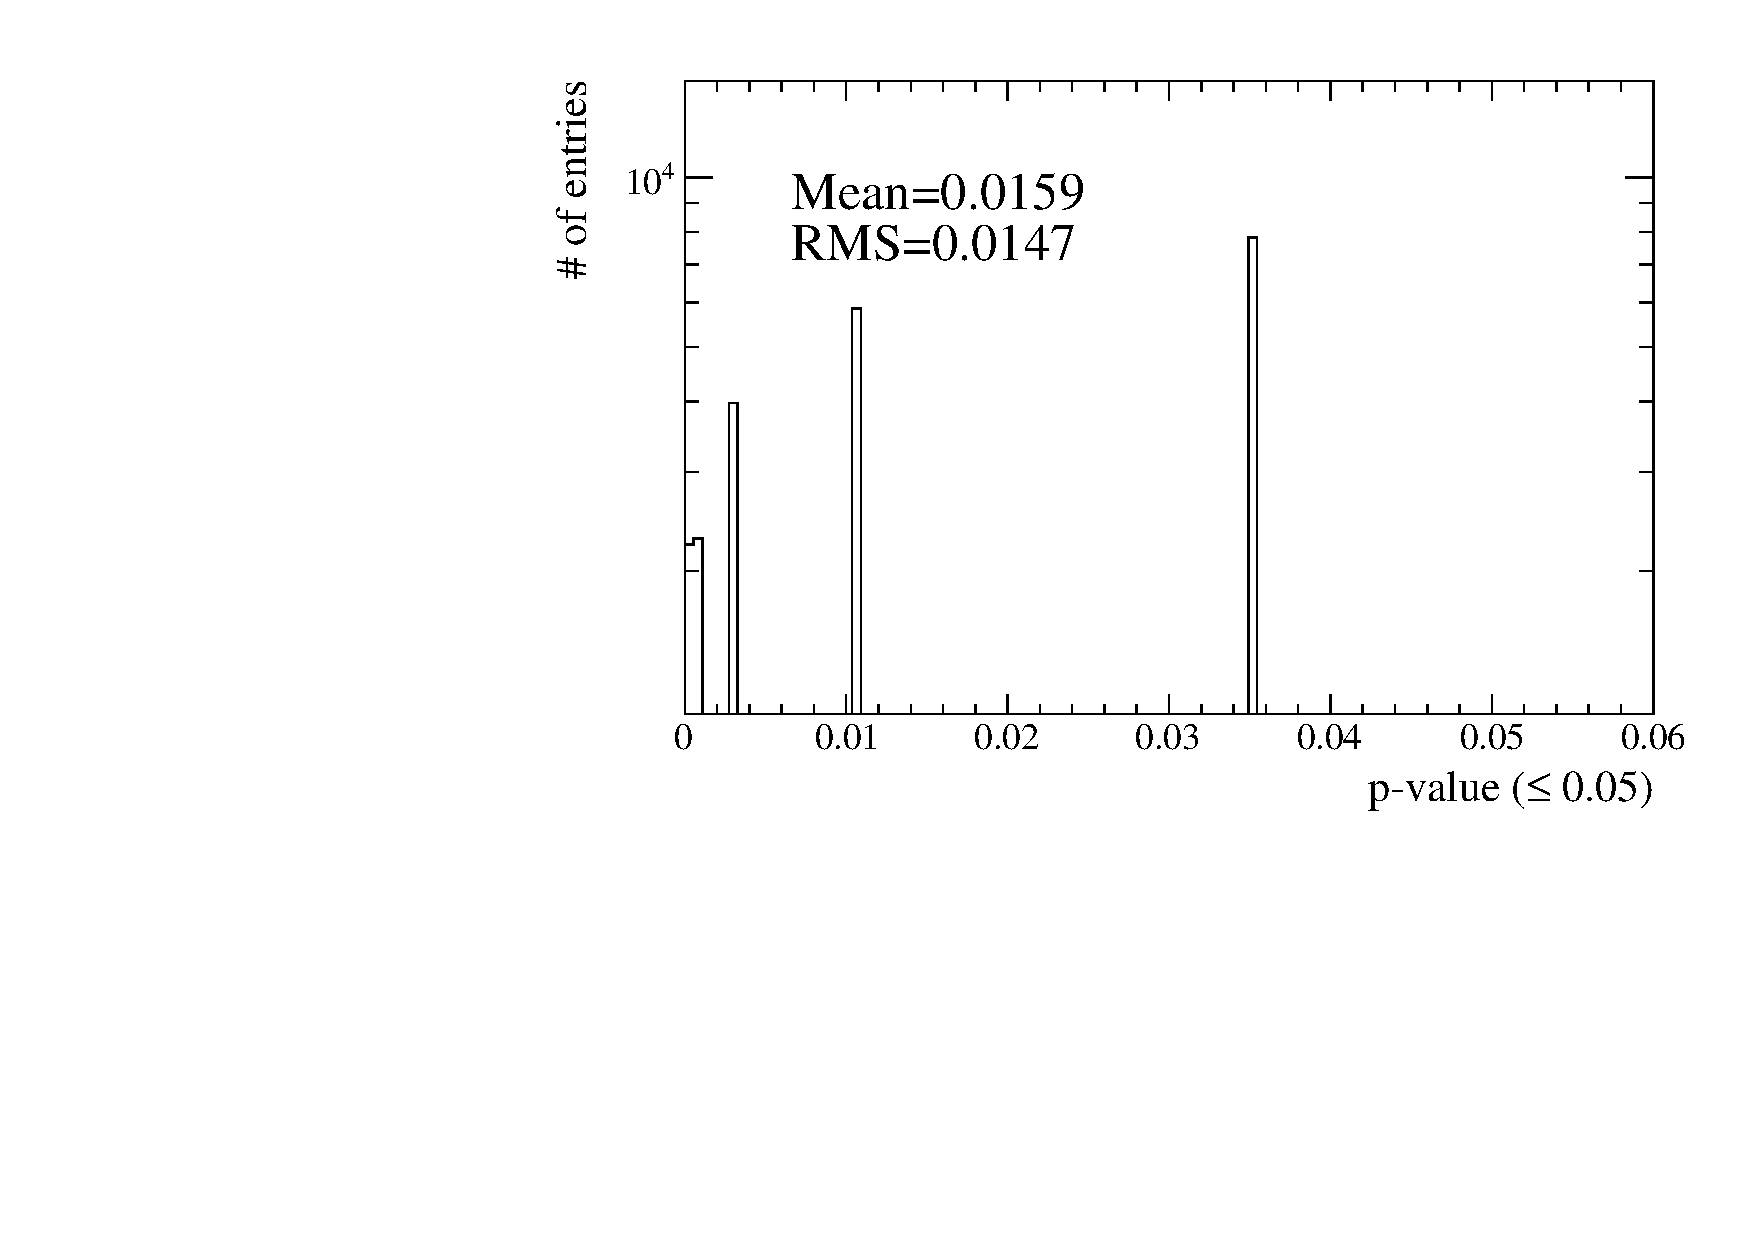
\includegraphics[width=0.48\linewidth]{./nuebar_plots/pvalue_mean/pvalue_fraction_4p0108E20POT/pvalue_rateonly_0p05_4p0108E20POT_50ktoys.pdf}
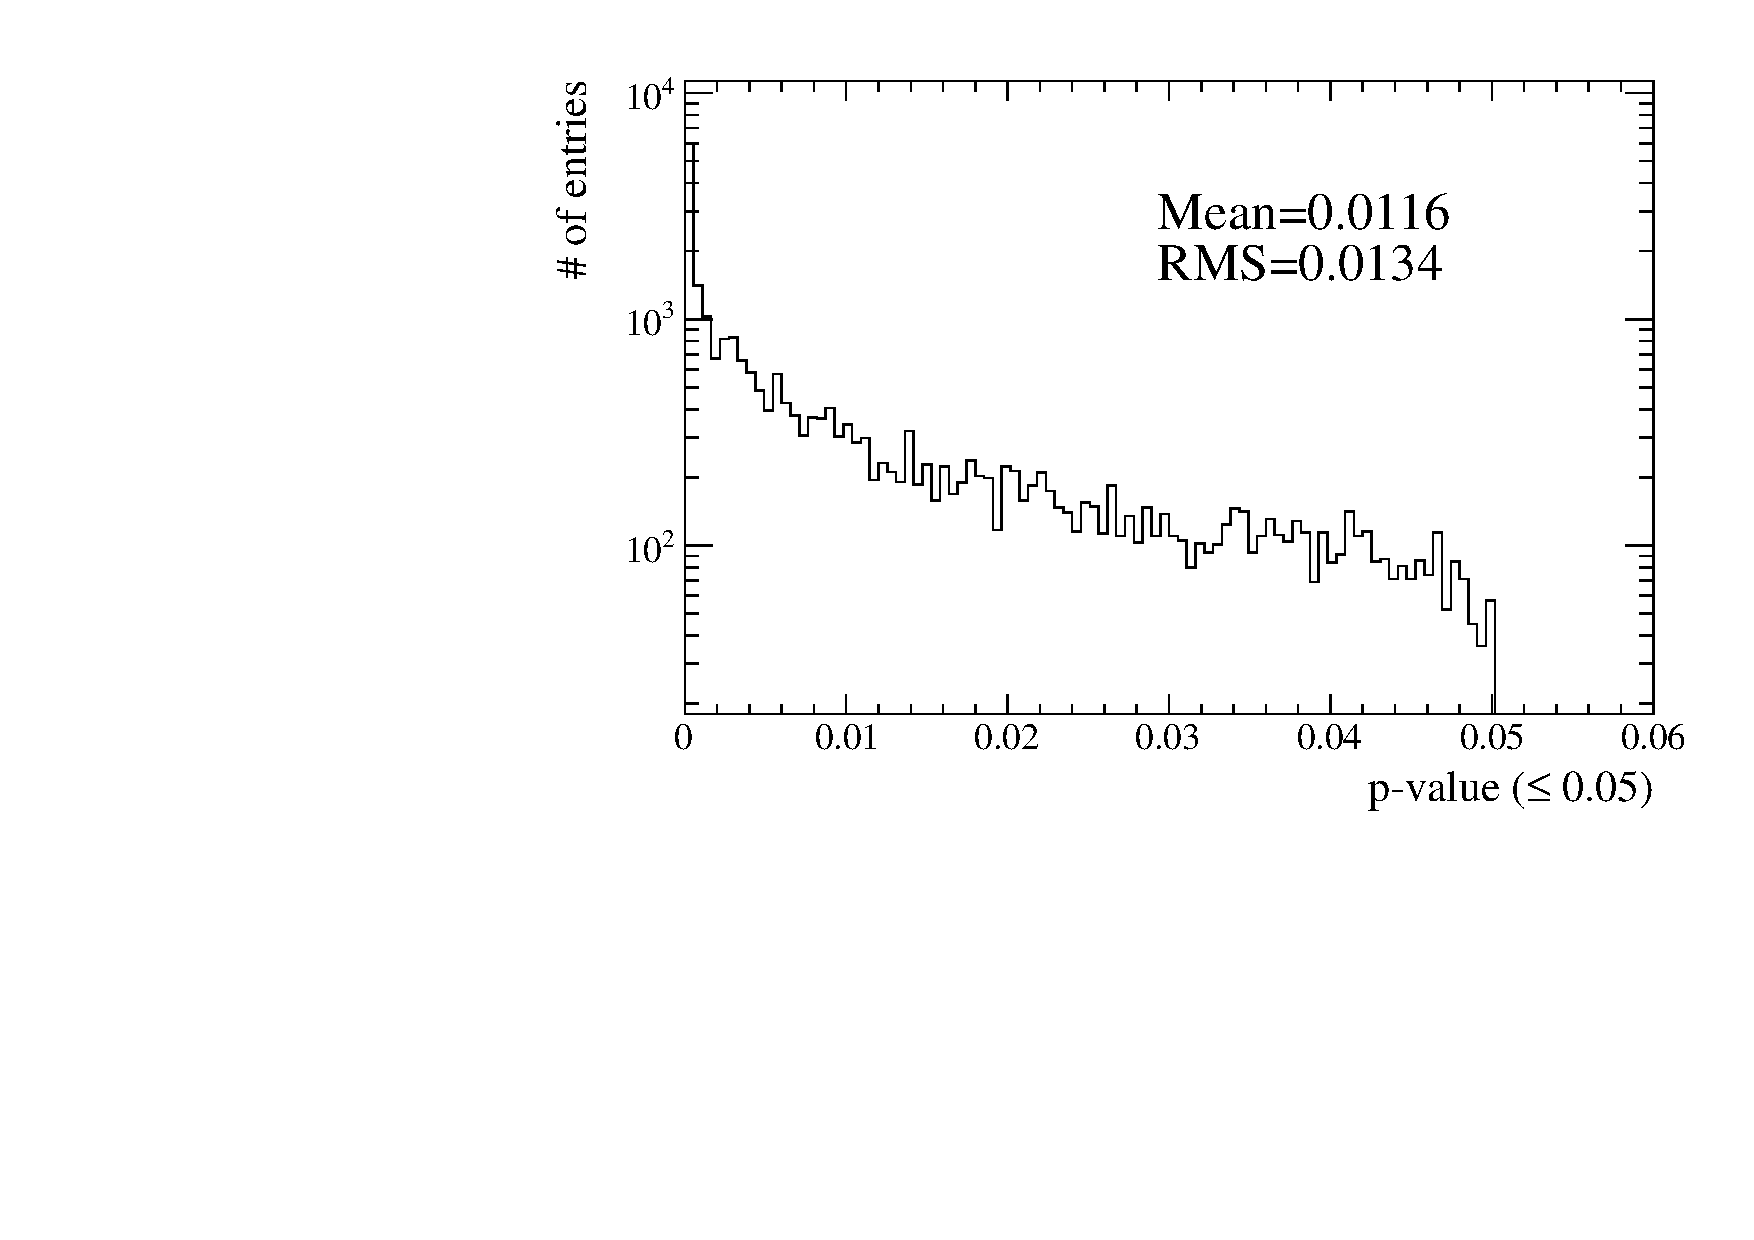
\includegraphics[width=0.48\linewidth]{./nuebar_plots/pvalue_mean/pvalue_fraction_4p0108E20POT/pvalue_rateshape_0p05_4p0108E20POT_50ktoys.pdf}
\caption {
The mean rate-only and rate+shape p-values, obtained considering only p-values smaller than 0.05 (0.10), are shown.
for 
\TotalPot POT.
%\FakePotLow POT.
\NumToysLarge toys are produced as described in Sec.~\ref{subsec:pvalue_mean}. 
Each entry corresponds to a different toy. 
}
\label{fig:pvalue_mean_0p05_lowpot}
\end{figure}

%\begin{figure}
%\center
%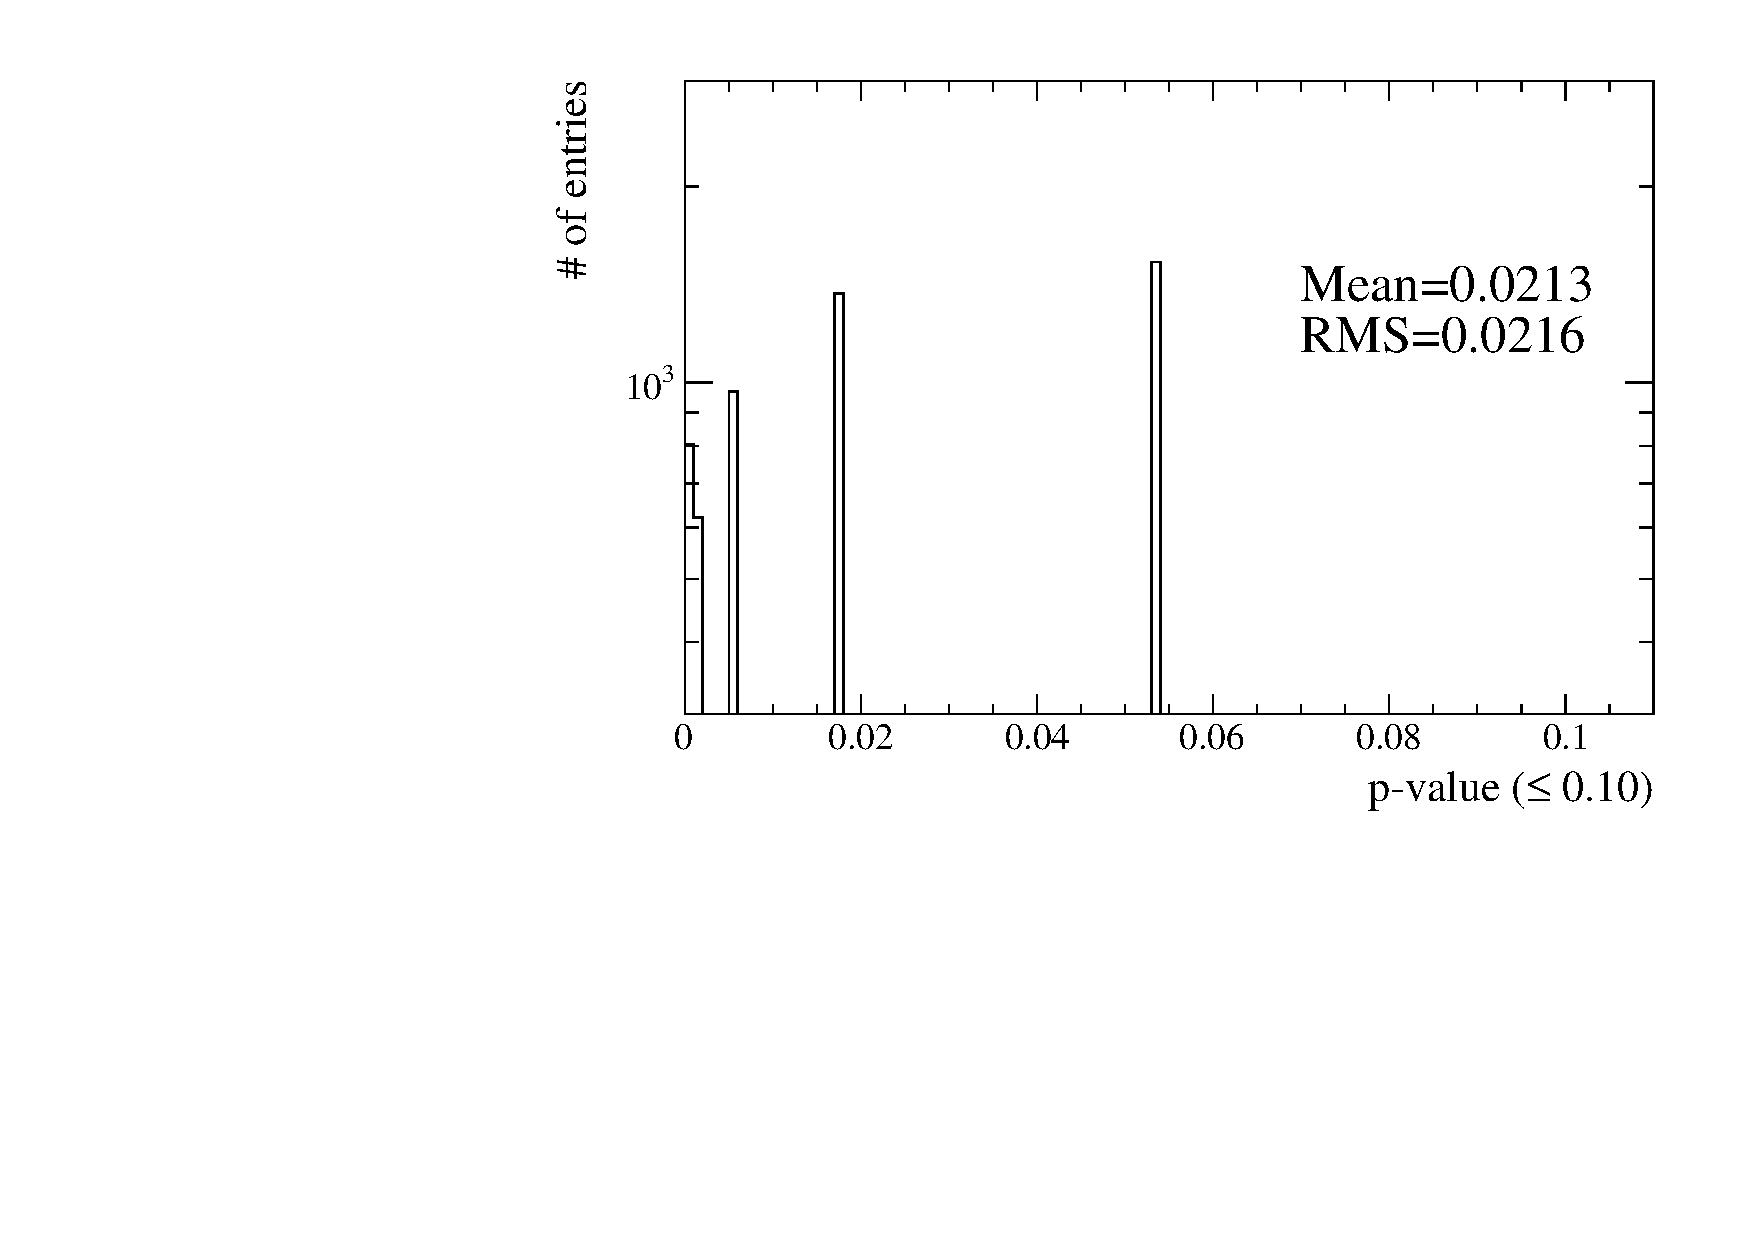
\includegraphics[width=0.48\linewidth]{./nuebar_plots/pvalue_mean/pvalue_fraction_4p5E20POT/pvalue_rateonly_0p10_4p5E20POT.pdf}
%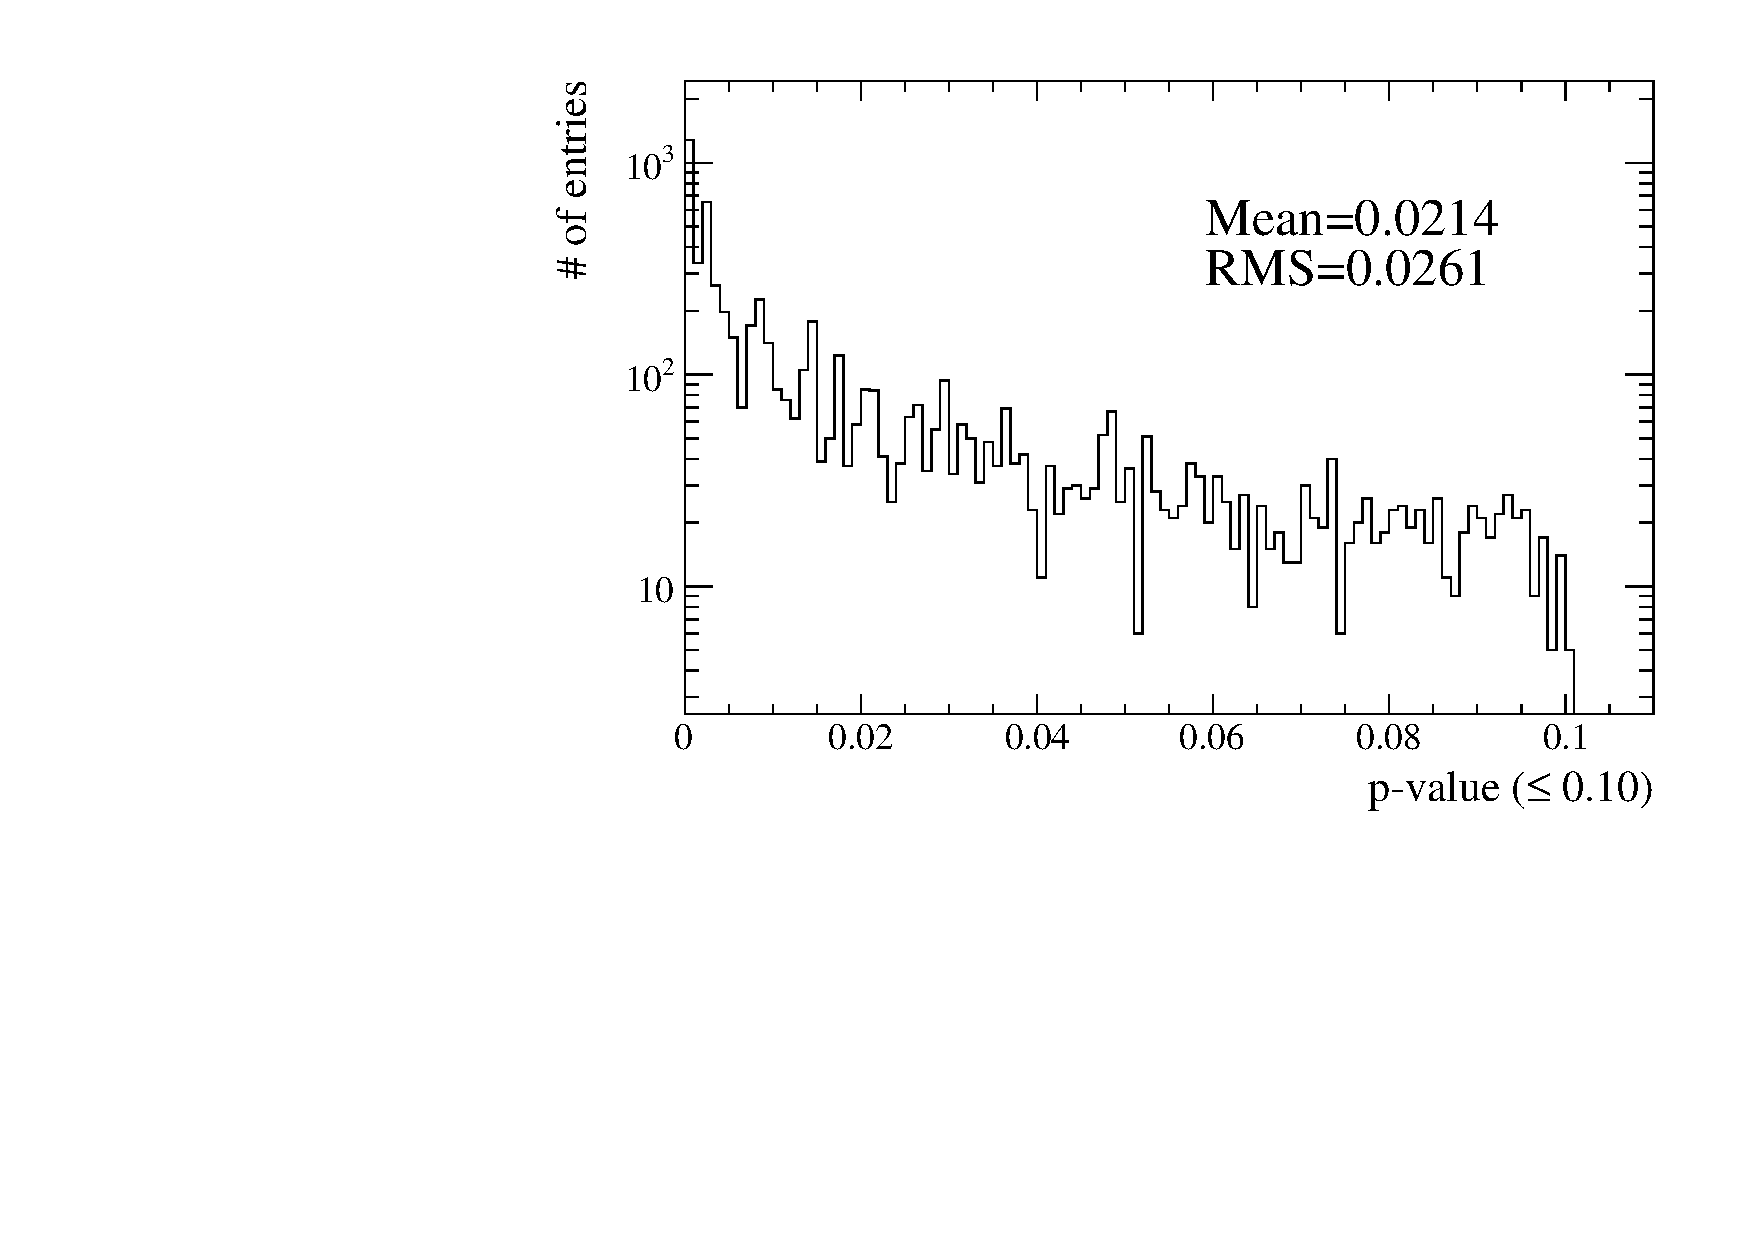
\includegraphics[width=0.48\linewidth]{./nuebar_plots/pvalue_mean/pvalue_fraction_4p5E20POT/pvalue_rateshape_0p10_4p5E20POT.pdf}
%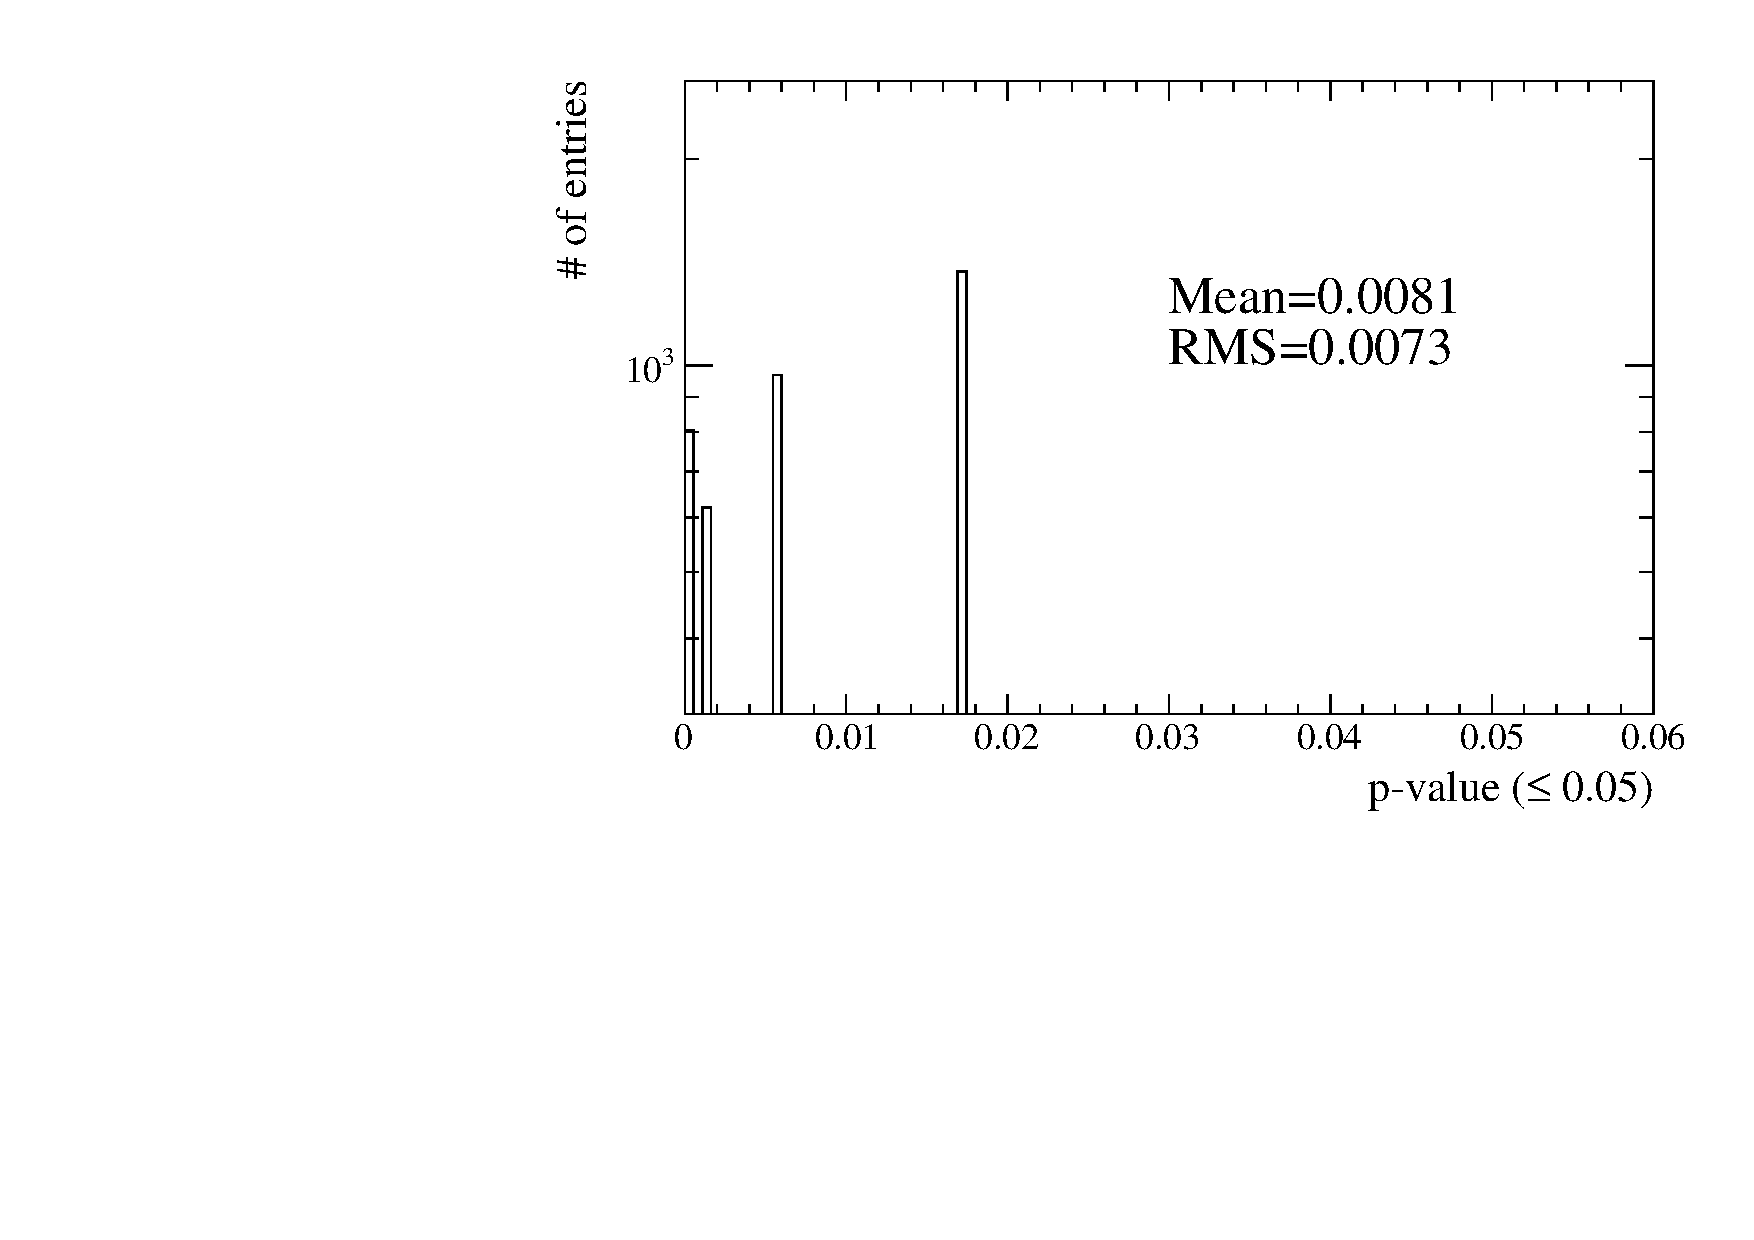
\includegraphics[width=0.48\linewidth]{./nuebar_plots/pvalue_mean/pvalue_fraction_4p5E20POT/pvalue_rateonly_0p05_4p5E20POT.pdf}
%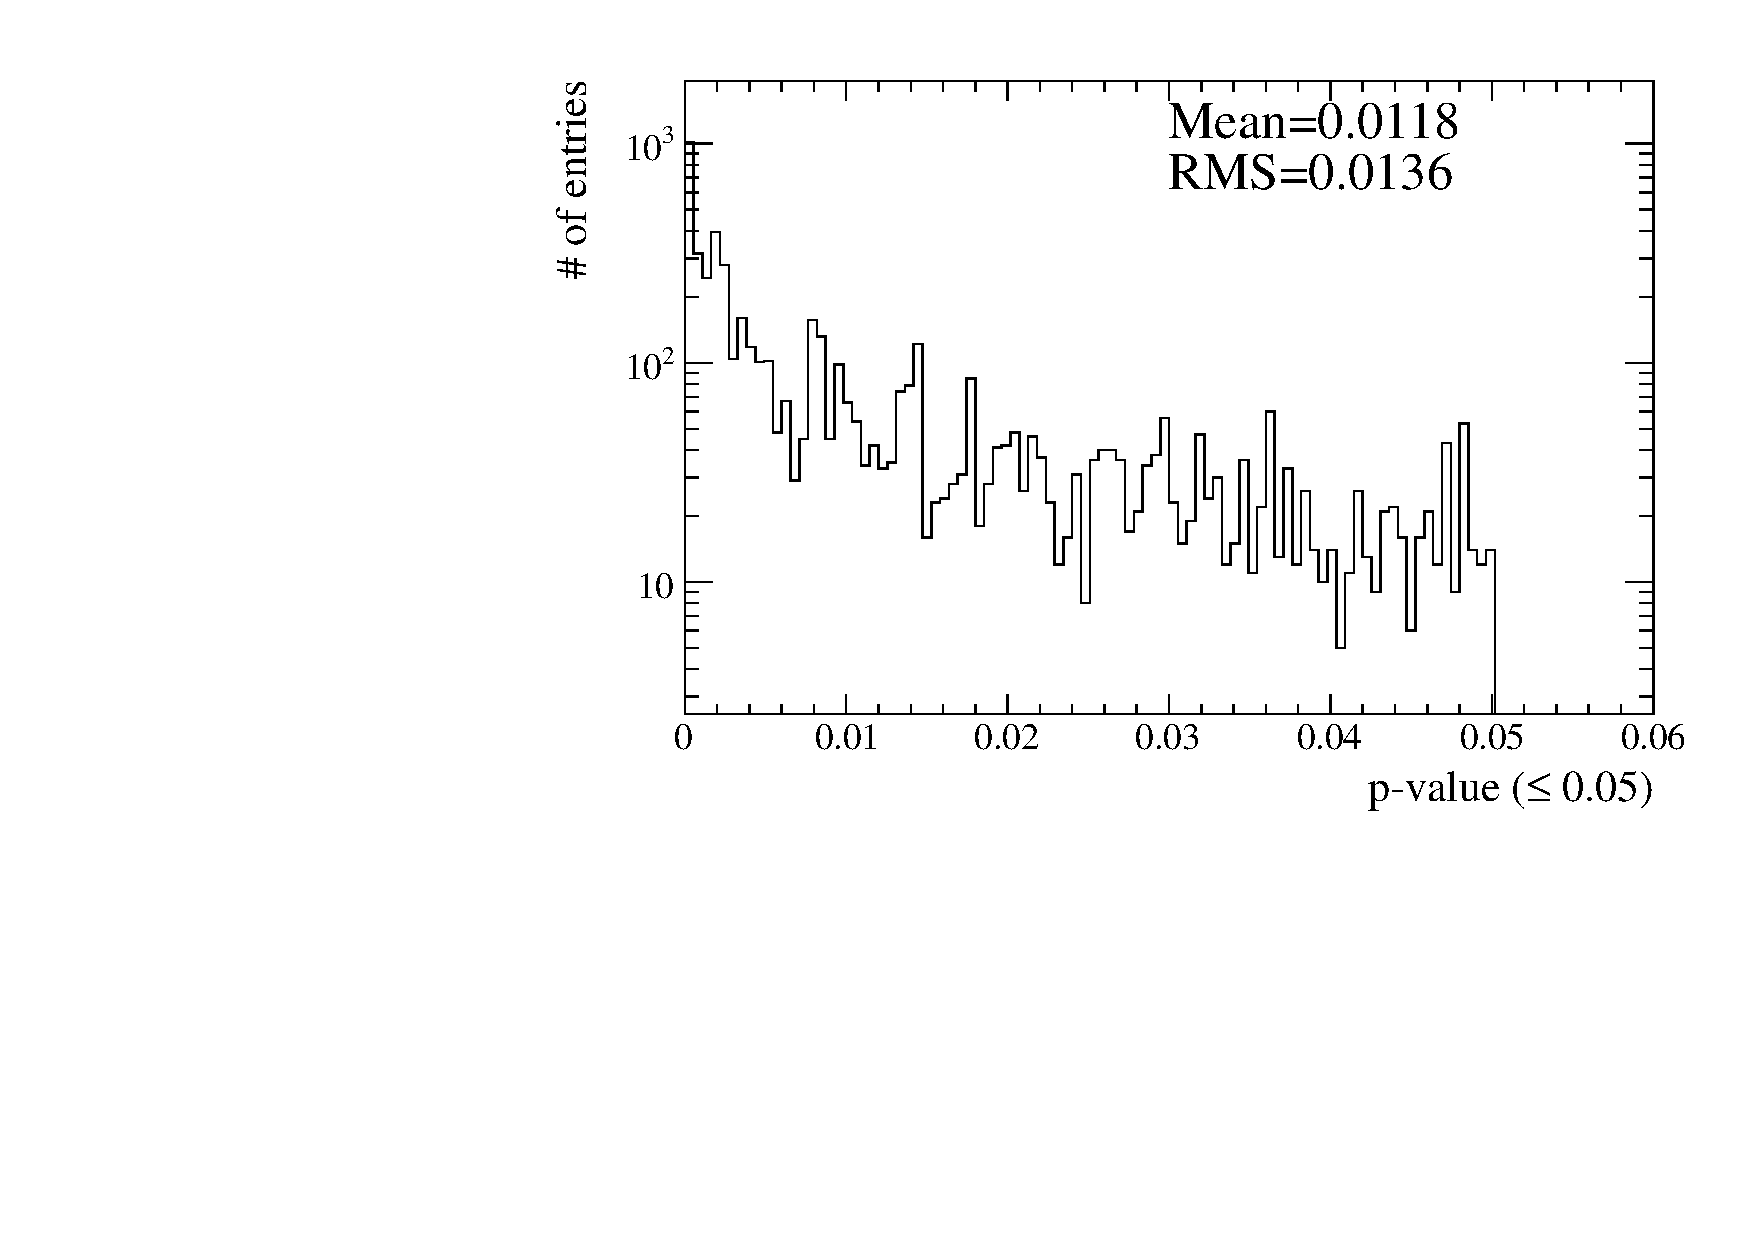
\includegraphics[width=0.48\linewidth]{./nuebar_plots/pvalue_mean/pvalue_fraction_4p5E20POT/pvalue_rateshape_0p05_4p5E20POT.pdf}
%\caption {
%The mean rate-only and rate+shape p-values, obtained considering only p-values smaller than 0.05 (0.10), are shown.
%for 
%\TotalPot POT.
%%\FakePotHigh POT.
%\NumToys toys are produced as described in Sec.~\ref{subsec:pvalue_mean}. 
%Each entry corresponds to a different toy. 
%}
%\label{fig:pvalue_mean_0p05_highpot}
%\end{figure}





In the mean rate-only and rate+shape p-values, obtained considering p-values with the 
condition that the number of observed events is larger than the expected background is shown.

\begin{figure}
\center
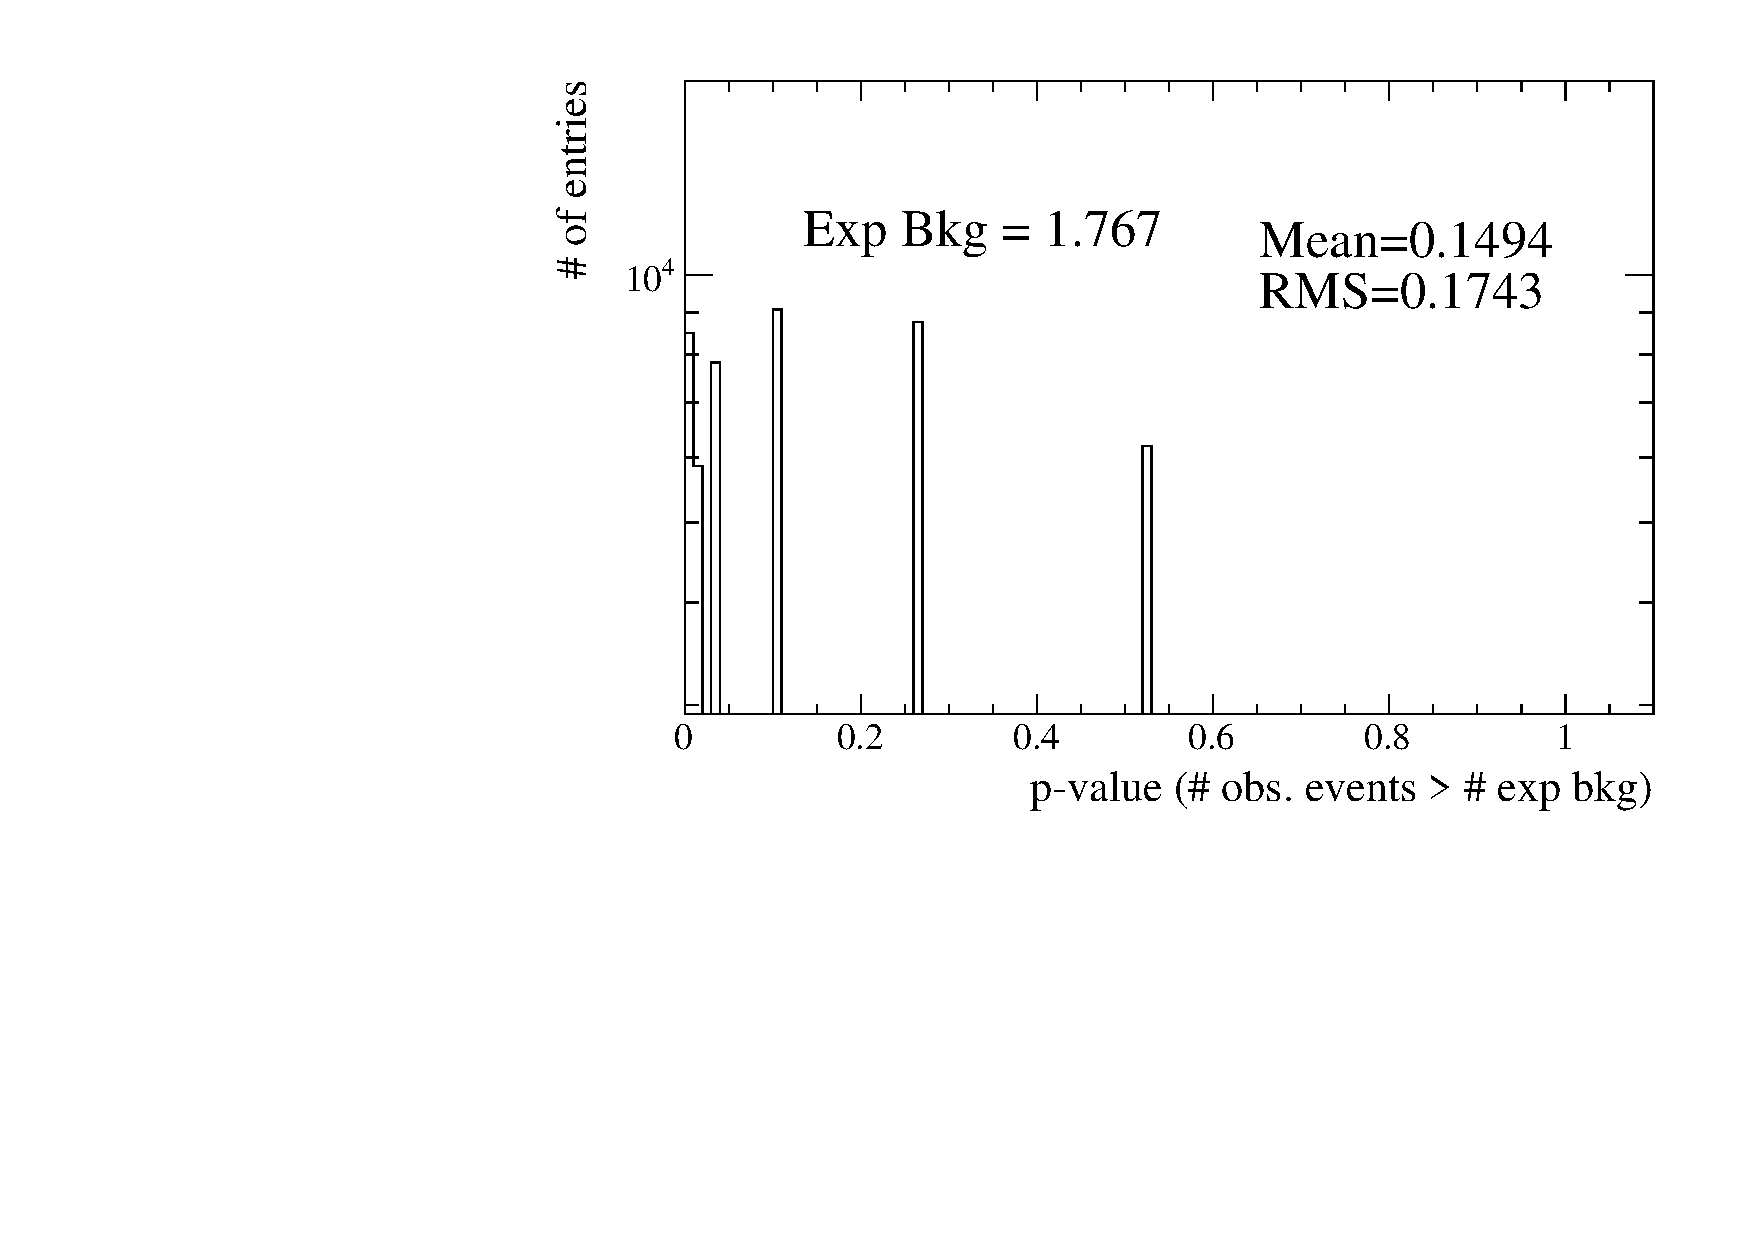
\includegraphics[width=0.48\linewidth]{./nuebar_plots/pvalue_mean/pvalue_bkg/pvalue_rateonly_bkg_4p0108E20POT_50ktoys}
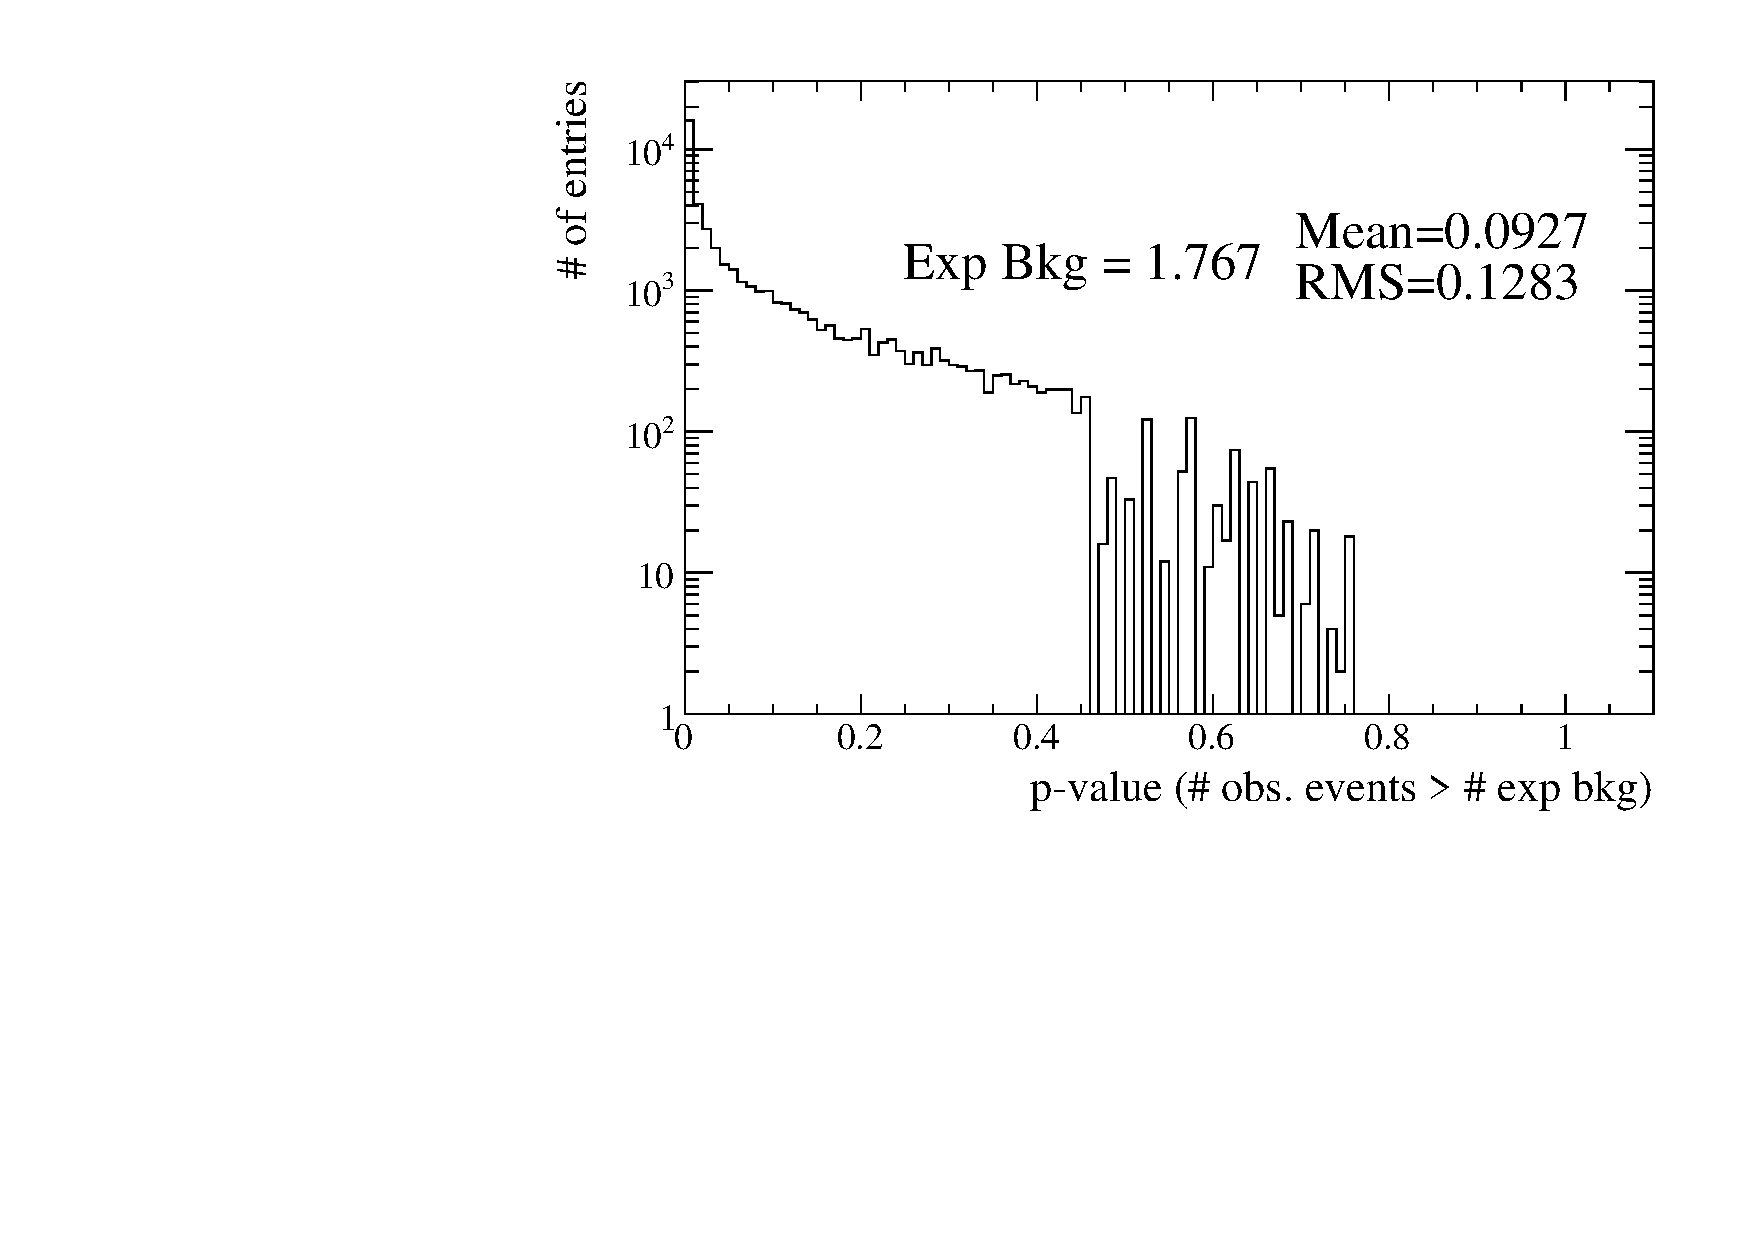
\includegraphics[width=0.48\linewidth]{./nuebar_plots/pvalue_mean/pvalue_bkg/pvalue_rateshape_bkg_4p0108E20POT_50ktoys}
%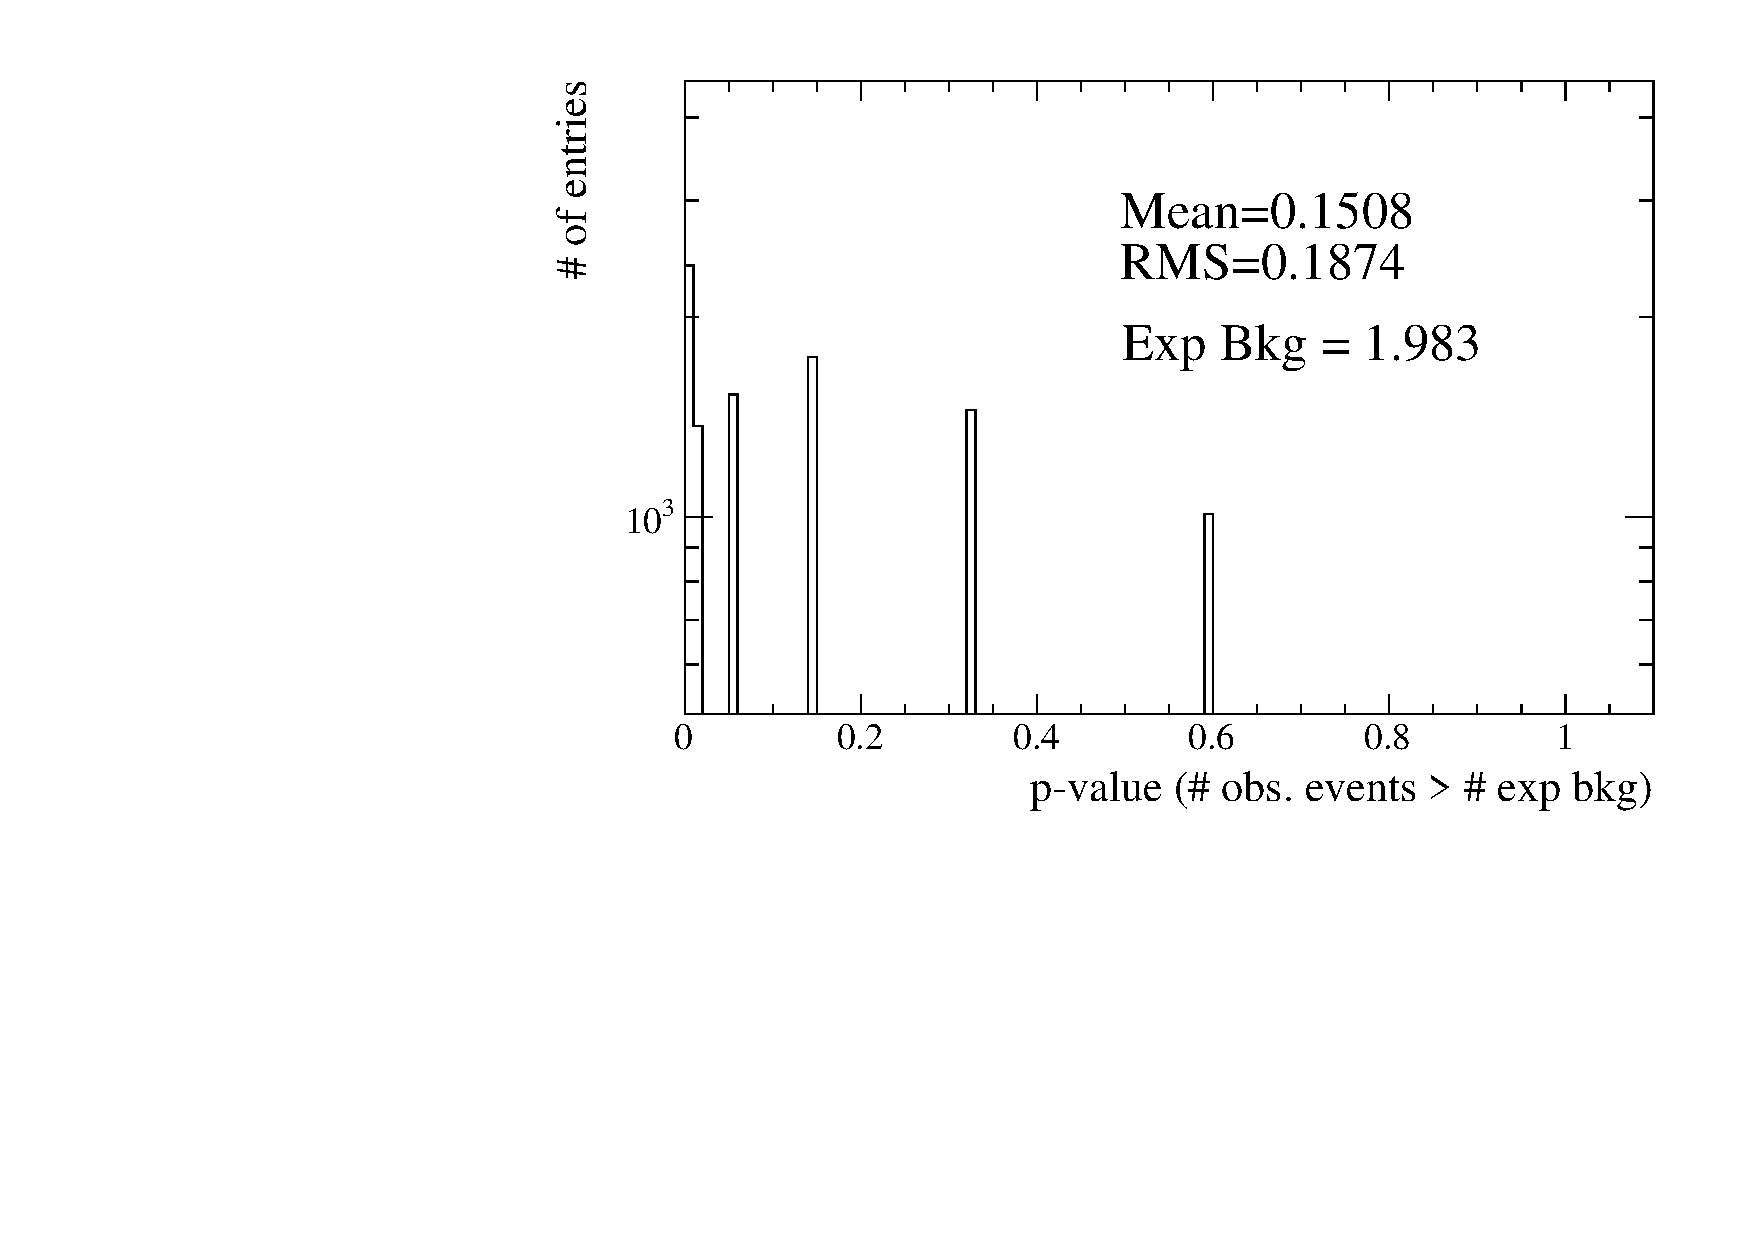
\includegraphics[width=0.48\linewidth]{./nuebar_plots/pvalue_mean/pvalue_bkg/pvalue_rateonly_bkg_4p5E20POT}
%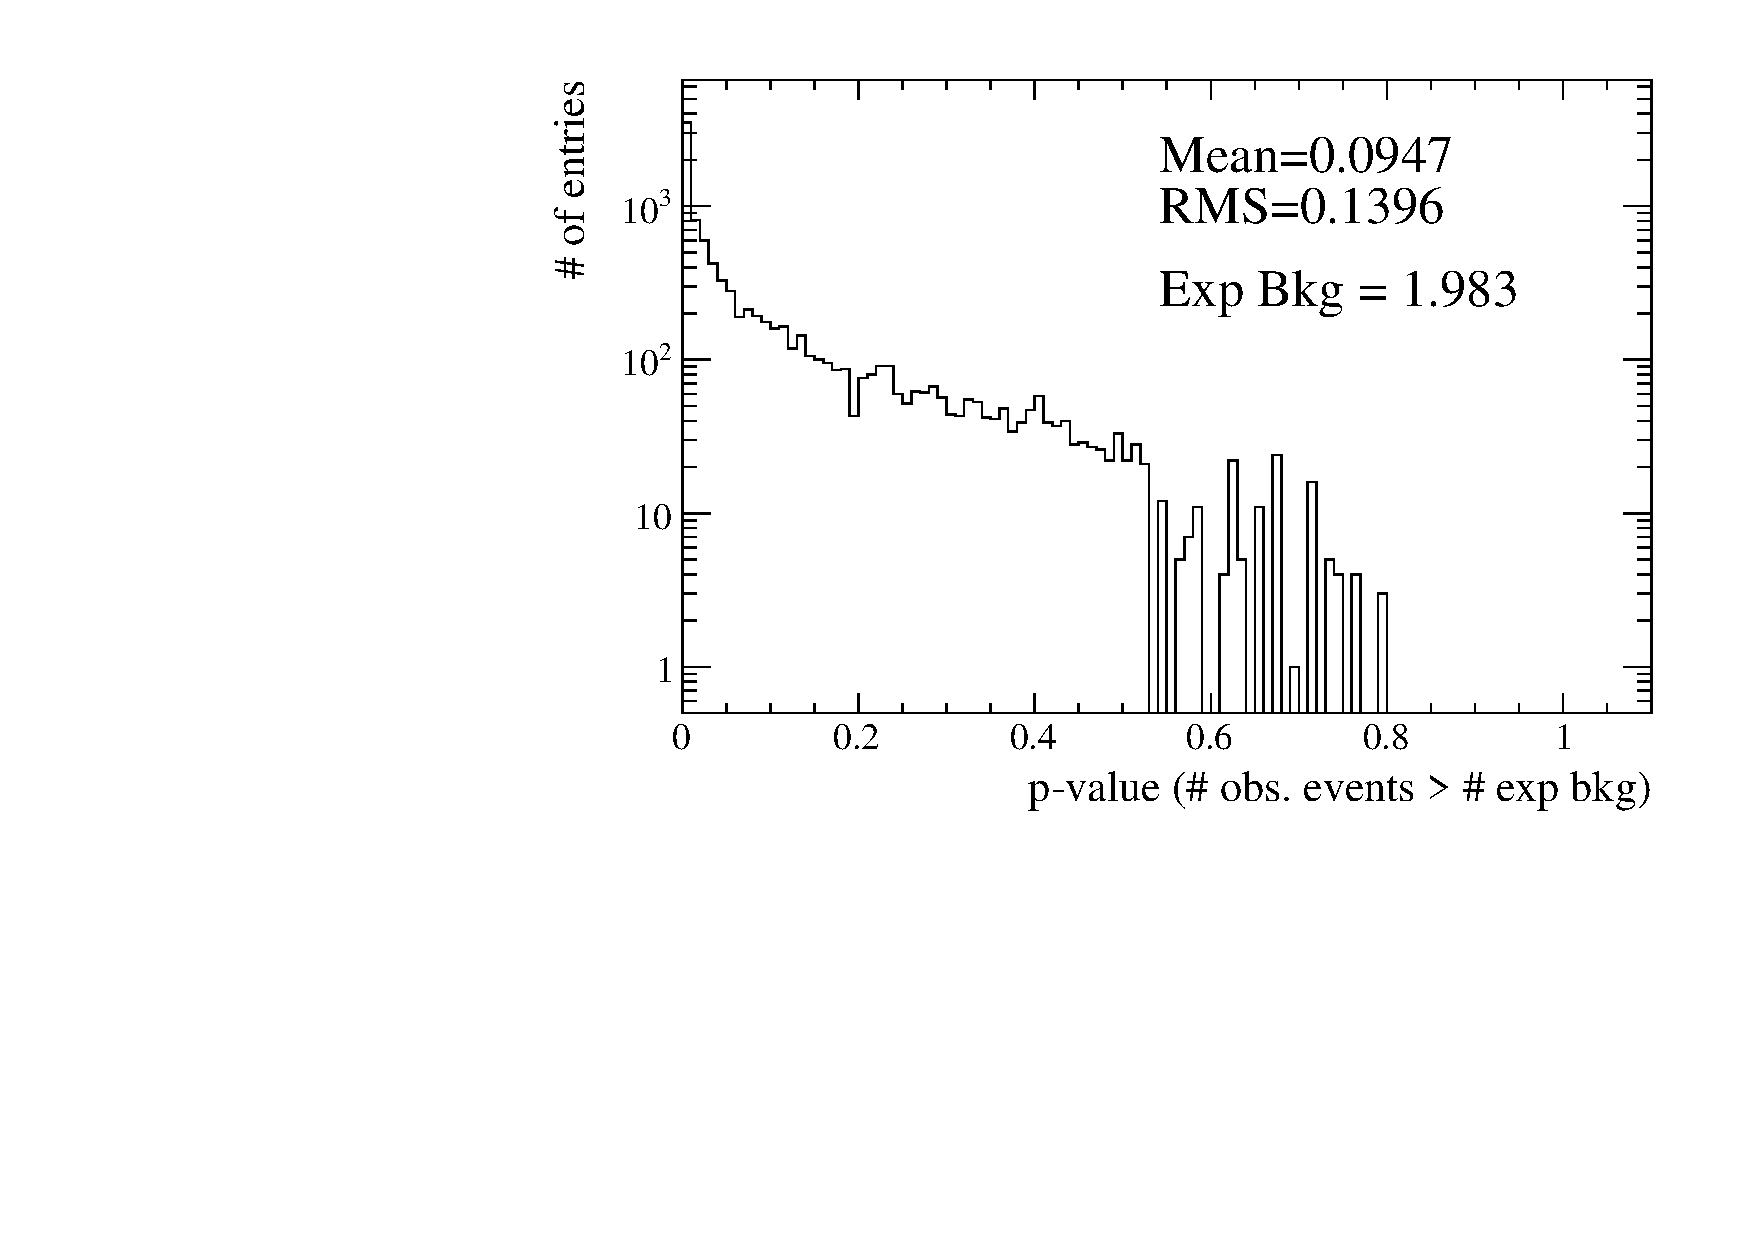
\includegraphics[width=0.48\linewidth]{./nuebar_plots/pvalue_mean/pvalue_bkg/pvalue_rateshape_bkg_4p5E20POT}
\caption {
The mean rate-only (left) and rate+shape (right) p-values, obtained considering p-values with the 
condition \# of observed events $>$ \# expected background is shown.
for
\TotalPot POT. 
%\FakePotLow POT (top) and \FakePotHigh POT (bottom).
\NumToysLarge toys are produced as described in Sec.~\ref{subsec:pvalue_mean}. 
Each entry corresponds to a different toy. 
}
\label{fig:pvalue_mean_bkg}
\end{figure}

















\clearpage


